\documentclass[11pt]{article}

% Change "review" to "final" to generate the final (sometimes called camera-ready) version.
% Change to "preprint" to generate a non-anonymous version with page numbers.
% \usepackage[preprint]{acl}
\usepackage[review]{acl}
\usepackage{listings}
% Standard package includes
\usepackage{times}
\usepackage{latexsym}
\usepackage{cuted}
\usepackage{enumitem}
% For proper rendering and hyphenation of words containing Latin characters (including in bib files)
\usepackage[T1]{fontenc}
% This assumes your files are encoded as UTF8
\usepackage[utf8]{inputenc}

% This is not strictly necessary, and may be commented out,
% but it will improve the layout of the manuscript,
% and will typically save some space.
\usepackage{microtype}

% This is also not strictly necessary, and may be commented out.
% However, it will improve the aesthetics of text in
% the typewriter font.
\usepackage{inconsolata}

% Including images in your LaTeX document requires adding
% additional package(s)
\usepackage{graphicx}

% Math and additional packages required by paper content
\usepackage{amsmath}
\usepackage{amssymb}
\usepackage{bm}
\usepackage{booktabs}
\usepackage{array}
\usepackage{caption}

\newcommand{\Vsw}{\mathbf{V}_{\!\textsc{SW}}}

\title{Values Are Not Enough: Situational Modifiers Shape Value-Based Decisions in LLMs and Humans}

\author{
  \textbf{Peddi Manognya}, 
  \textbf{Joshi Sayali Shripad}, 
  \textbf{Lokendra Mandloi}, 
  \textbf{Sandipan Dandapat} \\
  Indian Institute of Technology Hyderabad \\
  \small\texttt{\{cs24mtech12020, cs24mtech12003, cs24mtech11024\}@iith.ac.in} \\
  \small\texttt{sdandapat@cse.iith.ac.in}
}

\begin{document}
\maketitle

\begin{abstract}
\noindent
Personal values alone cannot fully explain moral decisions.
They are often treated as the main driver of moral choice, yet situational pressures can still shift actions when values are fixed. To study this effect, we introduce VISDA (\textbf{V}alue-\textbf{I}nformed \textbf{S}cenario- \textbf{D}riven \textbf{A}ctions), a dataset of 80 binary moral scenarios across various themes. Each scenario is augmented with eight situational modifier axes designed to capture contextual pressures on decision-making. Keeping value profiles constant, we evaluate three open-weight LLMs (Gemma 4 31B, Qwen 2.5 32B, LLaMA 3.1 8B), a utility-based mathematical baseline over 95 Schwartz profiles, and humans for their decisions under modifiers.
% ($N=50$; PVQ-21).
Each scenario is augmented with eight situational modifier axes designed to capture contextual pressures on decision-making, whereas LLMs reverse decisions (\textit{flips}) less frequently (2.03\%-8.92\%), with larger models showing greater sensitivity. Authority and self-preservation modifiers drive most flips and remain statistically significant after correction. Humans show a larger pooled shift ($|\Delta P(A)|=12.36\%$) and prioritize stakes and affective modifiers, while LLMs overweight personal-cost modifiers. This work reveals axis-level misalignment between human and LLM sensitivity to situational moral factors.
% \footnote{Code, dataset, and analysis pipeline: \url{https://github.com/Ardnekol/VISTA}.}
\end{abstract}

\section{Introduction}
\label{sec:intro}

\begin{figure}[t]
  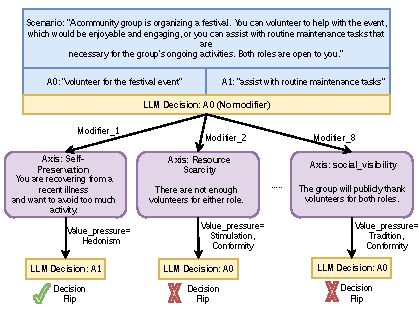
\includegraphics[width=1\columnwidth]{TDL.pdf}
  \caption{Schematic illustration of situation-driven decision flips. A fixed Schwartz value profile is paired with a baseline scenario and then independently augmented with Modifier axes. By comparing decisions before and after modifier insertion, we measures how contextual pressures alter model and human choices while holding values constant.}
  \label{fig:TDL}
\end{figure}


In psychology, values are often treated as principles that guide behavior across situations. One widely used framework is Schwartz’s value theory \citep{schwartz2012refined}, which organizes values along various dimensions. 
% such as openness-to-change vs. conservation and self-enhancement vs. self-transcendence. 
% These values, commonly measured using PVQ-21 \citep{schwartz2003proposal}, are frequently used to explain differences in moral and social decision-making. 
Compared with broader frameworks such as moral foundations theory \citep{haidt2012righteous}, Schwartz values map more directly onto action-level trade-offs.

Building on this view, recent work in psychology and LLM research assumes that a known value profile relates to behavior \citep{jiao2025ai, backmann2025ethics}. For example, valuing \textit{security} may favor cautious choices, while valuing \textit{benevolence} may favor helping at personal cost. Similarly, recent LLM studies show systematic behavioral shifts when value profiles are changed \citep{sauter2026between, guo2026counterfactual}.

However, situational context can strongly alter decisions even when values remain fixed \citep{nabizadeh2026large, sauter2026between, harry2026beyond, backmann2025ethics}. Decades of social psychology, especially the person-situation debate \citep{harry2026beyond, soni2025we, peterson2025context}, suggest that behavior depends not only on stable personality traits but also on immediate contextual pressures. A person who values honesty may still lie under pressure, and a loyal employee may still leave when the personal cost becomes too high. This suggests that values alone may not fully predict behavior.

% In psychology, values are often treated as stable principles that guide behavior across situations. One widely used framework is Schwartz’s value theory \citep{schwartz2012refined}, which organizes values along dimensions such as openness-to-change versus conservation and self-enhancement versus self-transcendence. These values, commonly measured using PVQ-21 \citep{schwartz2003proposal}, are frequently used to explain differences in moral and social decision-making. Compared with broader frameworks such as moral foundations theory \citep{haidt2012righteous}, Schwartz values map more directly onto action-level trade-offs.

% Personal values alone cannot fully explain moral decisions. Research in psychology and LLMs often assumes that a known value profile reliably predicts behavior \citep{jiao2025ai, harry2026beyond, backmann2025ethics}. For example, valuing security may favor cautious choices while valuing benevolence may favor helping at personal cost; recent LLM work likewise shows behavior shifts when value profiles are changed \citep{sauter2026between, guo2026counterfactual}.

% Situational context can strongly change decisions even when values remain fixed \citep{nabizadeh2026large, sauter2026between, backmann2025ethics}.
% Decades of social psychology, especially the person-situation debate \citep{harry2026beyond, soni2025we, peterson2025context}, show that human behavior depends not only on stable traits but also on immediate context.
% A person who values honesty may still lie under pressure.
% A loyal employee may still leave when the personal cost becomes too high.
% This means that values alone may not be enough to predict behavior.



% \begin{figure*}[t]
%   \centering
%   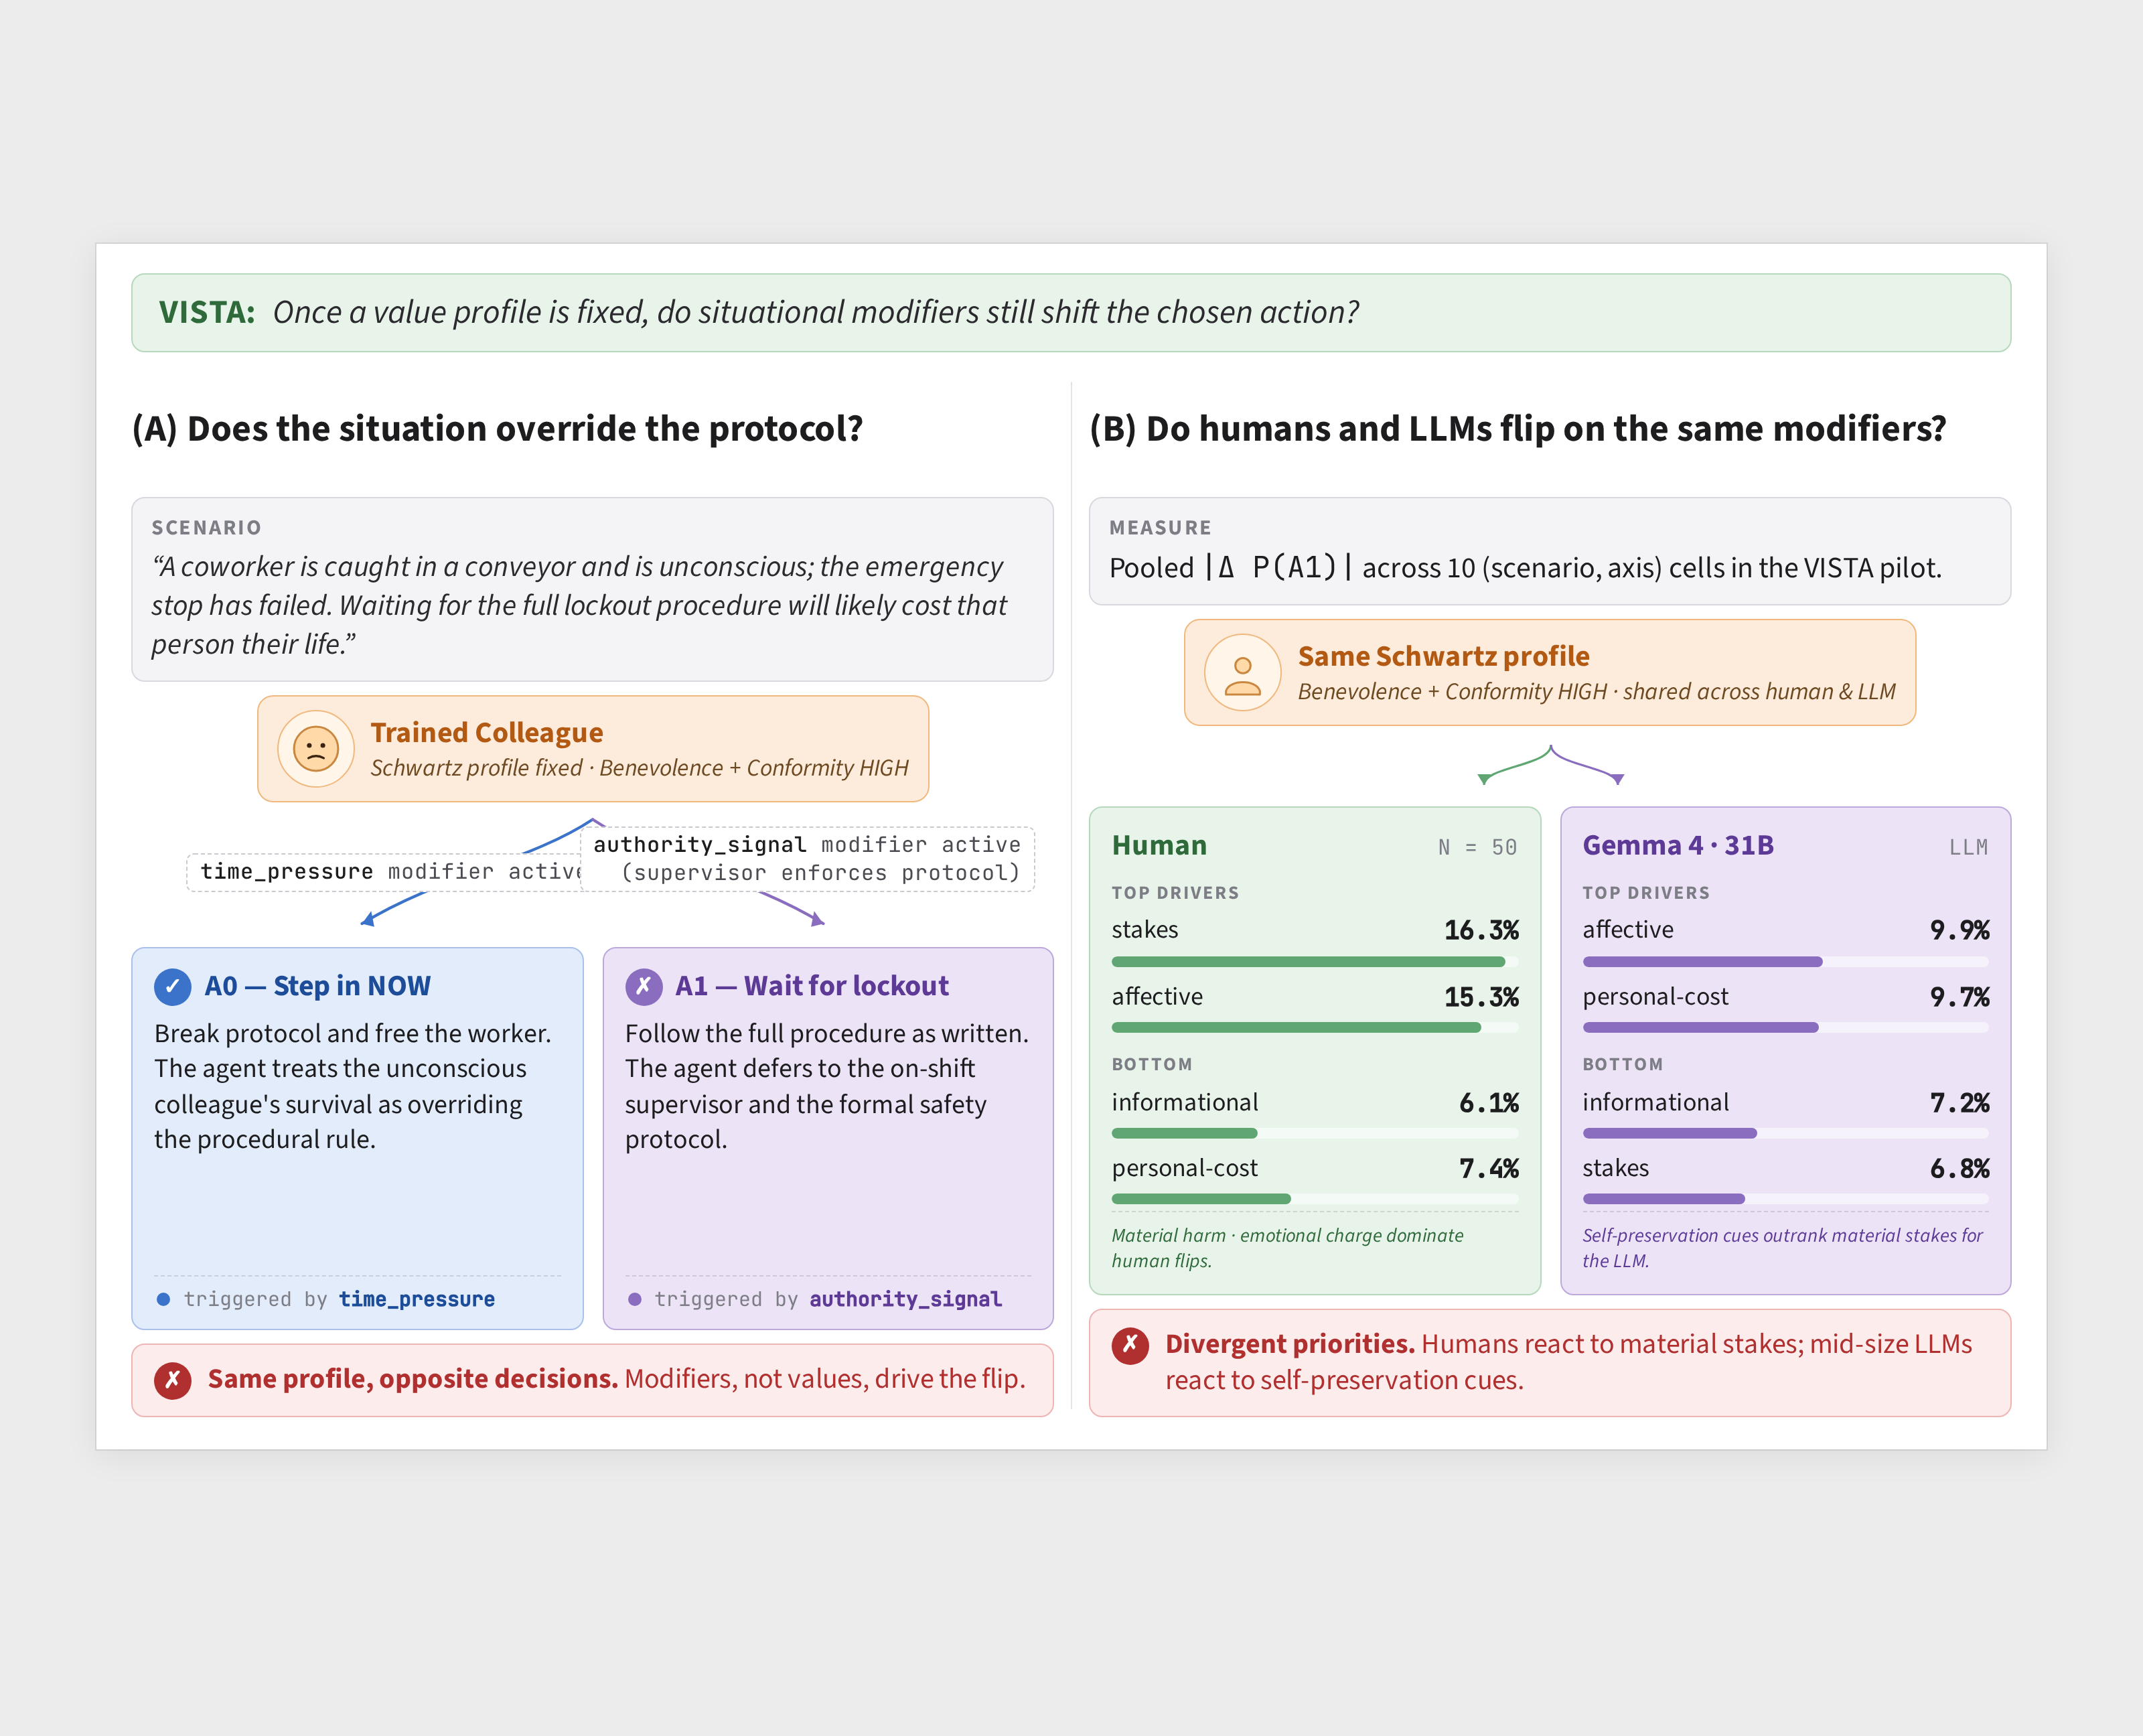
\includegraphics[width=0.85\textwidth]{vista_concept.png}
%   \caption{VISTA concept overview: a fixed Schwartz value profile is paired with a baseline scenario and its modifier-augmented variants; situation-driven behavioral change is measured via the \emph{decision-flip} metric across three open-weight LLMs, a utility-based mathematical baseline, and 50 human participants. \textbf{(A)}~With the Schwartz profile fixed, swapping the modifier flips the action: \texttt{time\_pressure}~$\!\to\!A_0$, \texttt{authority\_signal}~$\!\to\!A_1$. \textbf{(B)}~Per-axis $|\Delta P(A1)|$ shows divergent priorities-humans weight stakes/affective modifiers and  LLMs overweight self-preservation.}
%   \label{fig:concept}
% \end{figure*}

Current LLM evaluations of value-driven moral reasoning inadequately capture situational context, as most benchmarks only test whether different value profiles produce different decisions \citep{guo2026counterfactual, scherrer2023evaluating, jiao2025ai, mahajan2025mapping, schacht2025mapping}. Few studies examine whether a fixed value profile produces different actions when only the situational context changes~\citep{harry2026beyond, sauter2026between, backmann2025ethics}. Hence, it remains unclear whether LLMs act as stable value-driven agents or exhibit human-like context sensitivity.
% \citep{harry2026beyond, backmann2025ethics, jiaqi2025comparative}.

To study how situational changes affect decisions under a fixed value profile, we introduce \textbf{VISDA} (Value‑Informed Scenario‑Driven Actions), a dataset of 80 binary moral scenarios with systematically designed situational modifiers. As shown in Figure~\ref{fig:TDL}, each scenario pairs two actions with modifier sentences (e.g., emotional pressure, personal cost, social expectations, stakes), and situation-driven change is measured via a \emph{decision-flip} metric. Using matched Schwartz value profiles \citep{schwartz1992universals}, we evaluate a utility baseline, three open‑weight LLM families (LLaMA, Gemma, Qwen), and decisions of $50$ human participants of the survey. The effect of situational modifiers on altering decisions across LLMs is observed to be minimal: the utility baseline flips 19.93\%, whereas LLMs exhibit a flip rate less than 10\%. While LLMs detect modifiers sometimes, they redistribute pressure across modifier axes differently from humans. This shows that moral behavior cannot be fully explained by value profiles alone, as situational pressures substantially impact decisions.
% ; humans are more responsive to affective modifiers than current LLMs. 
%Overall, value profiles alone do not fully predict moral behavior.
The primary contributions of the paper includes:
\begin{itemize}[leftmargin=*,noitemsep, topsep=0pt]
    \item We introduce a new evaluation framework for measuring how situational context alters moral decisions under fixed value profiles.
    \item We propose the decision-flip metric as a direct measure of situation-driven behavioral change.
    \item We construct a controlled dataset of 80 moral-decision scenarios with systematically designed situational modifiers.\footnote{The dataset and code will be publicly released upon acceptance.}
    \item We compare humans, utility-based baselines, and multiple LLMs under a shared value framework to analyze how value profiles and situational modifiers influence decision-making.
\end{itemize}


%This paper makes four contributions.  
%First, we introduce a controlled dataset.
% of 80 moral-decision situations with systematically designed situational modifiers.  
%Second, we compare situational sensitivity across various systems.
% mathematical baselines, LLMs, and human participants using the same value framework.  
%Third, we propose the decision-flip metric as a direct way to measure situation-driven behavioral change. 
%Fourth, we analyze the effects of value profiles and situational modifiers on LLM decision-making. 
% Fourth, we provide evidence that value profiles are necessary but insufficient predictors of moral behavior in both humans and LLMs.  

% The remainder of the paper is organized as follows. Section~\ref{sec:related} reviews prior work on values, moral reasoning, and situational effects in humans and LLMs. Section~\ref{sec:method} describes the construction of VISDA dataset, value representation, experimental setup, and the evaluation pipeline. Section~\ref{sec:analysis} reports decision-flip results and human-LLM agreement analyses.
% Finally, Section~\ref{sec:conclusion} presents conclusions and future directions, followed by limitations and ethics statements.

\section{Related Work}
\label{sec:related}

\textbf{Values, traits, and behavior.}
Schwartz's refined value theory~\citep{schwartz2012refined} organizes 19 basic values on a circumplex spanning openness to change, conservation, self‑enhancement and self‑transcendence.
% For tractability we adopt a reduced 10‑value representation (see Section\ref{sec:method}).
The Portrait Values Questionnaire (PVQ‑21)~\citep{schwartz2003proposal} is a validated short instrument for assessing these values. 
% Although Haidt's moral foundations theory offers a complementary lens \citep{haidt2012righteous}, we use Schwartz because it maps directly to action‑level choices. 
Social psychology has long debated whether stable dispositions or situational context better predict behavior \citep{mischel1968personality, ross1991person}.
% ; recent work reports that a large share of variance is within‑person (e.g., 74\% in \citealp{harry2026beyond}).
By contrast, LLMs tend to be state‑blind and respond mainly to trait‑level prompts, and \citet{soni2025we} reports that situational context can alter responses in ways dispositional profiles alone do not capture.

\textbf{Value-driven LLMs.}
Recent work has examined whether LLMs can follow prescribed value profiles. \citet{sorensen2024value} introduce the \emph{Value Kaleidoscope} corpus, which maps values, rights, and duties to actions. \citet{abdulhai2023moral} and \citet{scherrer2023evaluating} probe the moral beliefs implicit in pretrained LLMs, finding that encoded preferences are consistent across scenarios and that closed-source models tend to agree with one another. 
\citet{kang2023values} demonstrate that injecting Schwartz value vectors into prompts changes downstream stance prediction. 
\citet{guo2026counterfactual} shows that steering value priorities via counterfactual reasoning produces predictable changes in model output, and \citet{jiao2025ai} finds that assigning good or evil personality profiles produces systematic shifts in moral judgment even under time pressure. 

\textbf{Situational and contextual effects.}
\citet{santurkar2023whose} and \citet{durmus2023globalopinionqa} show that LLM outputs shift under demographic or geographic priming, suggesting that factors beyond the explicit value profile can affect the chosen action. More directly, \citet{sauter2026between,nabizadeh2026large,backmann2025ethics} find that contextual framing, opponent behavior, survival risk, and broader ethical themes can all change moral judgments even when the underlying model is unchanged. Together, these results indicate that situational modifiers independently shape moral decisions beyond what value profiles alone predict.
\citet{peterson2025context} frames this as person-situation dynamics in LLM alignment, echoing classic social-psychology findings that behavior depends jointly on stable dispositions and immediate context.

\textbf{Moral reasoning benchmarks.}
Several benchmarks evaluate LLM moral reasoning at scale. \citet{samway2025language} analyze reasoning traces across 600+ trolley problems,
classifying outputs by consequentialist and deontological patterns. \citet{mahajan2025mapping}\ encode responses to
ethical dilemmas into an eleven-dimensional normative profile but
acknowledge only limited framing variation across scenarios. \citet{schacht2025mapping} provides a mechanistic
analysis of ethical decision-making in LLMs, examining situational cues
but without holding value profiles fixed.
ETHICS \citep{hendrycks2021ethics} and MoralStories \citep{emelin2021moral}
provide labeled corpora for moral judgment but do not systematically
vary situational modifiers under a fixed value profile. \citet{jiaqi2025comparative} find that LLM personality traits are dynamic and input-driven
rather than stable, suggesting that
current evaluation designs may underestimate situational sensitivity.

% The most closely related work to ours is \citep{harry2026beyond}, which introduces \emph{Chameleon}: a large observational dataset of contextual psychological profiles from Reddit. Their Latent State-Trait analysis shows that most variance is within-person and that LLMs are largely \emph{state-blind} under different state framings of the same user. We agree with that conclusion, but this work answers a different question: instead of inferring context from natural posts, we \emph{manipulate} one situational modifier at a time while holding the Schwartz value profile fixed. We also measure context sensitivity across various systems. This lets us identify not just whether models are state-blind, but which situational pressures they mis-weight relative to humans.

The work most closely related to ours is \citet{harry2026beyond}, which introduces \emph{Chameleon}, a large observational dataset of contextual psychological profiles from Reddit. Whereas their study analyzes naturally occurring contextual variation, our work uses controlled interventions that manipulate one situational modifier at a time while holding the Schwartz value profile fixed. This design allows us to identify not just whether models are state-blind, but also how they differentially calibrate situational pressures relative to humans.

\section{Data Curation}
\label{sec:method}

\subsection{Value Representation}
\label{sec:value-rep}

We adopt classic Schwartz's theory with $10$ universal value dimensions as in \citep{schwartz1992universals}. Each value takes a binary state $\in \{0,1\}$ (low or high), yielding a value vector $\Vsw \in \{0,1\}^{10}$. Although the full space contains \(2^{10} = 1024\) possible value profiles, we evaluate a curated subset of $95$ representative profiles selected through a semi-automated curation process to ensure diversity across value combinations. The complete list is provided in Appendix~\ref{app:profiles}.

\subsection{The VISDA Dataset}
\label{sec:dataset}

VISDA is built around five linked components: \emph{themes}, \emph{scenarios}, \emph{modifiers}, \emph{value profiles}, and \emph{profile descriptions}.
Themes, scenarios and modifiers are generated through prompts, followed by manual verification to keep only items that are plausible and consistent with the dataset design.
The exact prompts used to generate these components are given in Appendix~\ref{app:dataset}.
% The \emph{eight modifier axes} are predefined situational pressures drawn from established socio-psychological constructs and each modifier instantiates one familiar kind of context (e.g., authority, scarcity, or time pressure). For value profiles, we enumerate all binary value vectors, remove any profiles that contain mutually antagonistic values (for example, Power-Universalism, Achievement-Benevolence, or Openness-to-Change-Conservation), and retain a curated subset. For profile descriptions, we prompt an LLM to turn each binary value vector into a short natural-language description and then manually check the result for accuracy. 
Table~\ref{tab:visda_sample} shows one concrete chain of data spanning all five components, which serves as a running example throughout the paper.

\begin{table*}[t]
\centering
\footnotesize
\setlength{\tabcolsep}{4pt}
\begin{tabular}{p{0.16\linewidth} p{0.78\linewidth}}
\toprule
\textbf{Component} & \textbf{Sample entry} \\
\midrule
Theme & \texttt{TH004} — \emph{balancing personal enjoyment and obligations}; primary quadrant: Openness to Change; secondary quadrant: Conservation; potential value tensions: \{(Hedonism, Conformity), (Stimulation, Tradition)\}. \\
\addlinespace
Scenario & \texttt{SC004\_2} — A community group is organizing a festival. You can volunteer to help with the event, which would be enjoyable and engaging, or you can assist with routine maintenance tasks that are necessary for the group's ongoing activities. Both roles are open to you. $A_0$: volunteer for the festival event $A_1$: assist with routine maintenance tasks. Latent value tensions inherited from \texttt{TH004}. \\
\addlinespace
Modifier & \texttt{MOD\_SC004\_2\_01} — axis: \emph{self\_preservation}; modifier\_text: ``\emph{You are recovering from a recent illness and want to avoid too much activity.}''; expected\_value\_pressure: \{Hedonism\}. \\
\addlinespace
Value profile & \texttt{VSW\_037} — binary vector $[0,0,0,1,1,1,1,0,1,1]$ over (Self-Direction, Stimulation, Hedonism, Achievement, Power, Security, Conformity, Tradition, Benevolence, Universalism); active\_values\_count = 6. \\
\addlinespace
Profile description & ``You strongly value achievement and demonstrating competence. You value power and the ability to influence others. \ldots You strongly value universal concern for others.'' (10 sentences, one per Schwartz value, LLM-generated and reviewed.) \\
\bottomrule
\end{tabular}
\caption{One concrete row of VISDA, traced from theme down to the natural-language profile description that is shown to the LLM. The same five-component structure repeats for every scenario-modifier-profile combination in the dataset.}
\label{tab:visda_sample}
\end{table*}

\paragraph{(i) Themes:} A theme is a short moral or social setting designed to create tension between two of Schwartz's four higher-order quadrants: \emph{Openness-to-Change}, \emph{Self-Enhancement}, \emph{Conservation}, and \emph{Self-Transcendence} \citep{schwartz1992universals}. Each theme is tagged with a primary and a secondary quadrant showing which parts of the circumplex the tension spans (e.g., the theme \texttt{TH004} (\emph{balancing personal enjoyment and obligations}) in Table~\ref{tab:visda_sample} pits between the higher order values of \emph{Openness to Change} against \emph{Conservation}, with potential value tensions such as \{(Hedonism, Conformity), (Stimulation, Tradition)\}). The final set of themes includes resource allocation, workplace dynamics, recognition, personal choice, and leader succession. For each theme, \texttt{potential\_value\_tensions} are also listed which specify the Schwartz-value pairs that motivate the theme with underlying moral tension.

%The final set of themes is: 
%\begin{enumerate}[leftmargin=2em,nosep]
%  \item Resource allocation
%  \item Workplace
%  \item Recognition
%  \item Personal Choice
%  \item Leader Succession
%\end{enumerate}  
%\texttt{potential\_value\_tensions} are also listed for each theme, that specify the Schwartz-value pairs that motivate the theme.

\paragraph{(ii) Scenarios:} 
Scenarios instantiate a theme as a concrete decision-making situation involving an actor and competing actions. Each theme is expanded into two scenarios, giving 10 base scenarios. Generated scenarios satisfy four constraints:

\begin{enumerate}[label=(\alph*),leftmargin=2em,itemsep=0pt,topsep=2pt,parsep=0pt]
  \item Both actions must be plausible and socially acceptable.
  \item The two actions must reflect different \emph{value priorities} rather than different outcome quality (e.g., innovation vs.\ tradition).
  \item Wording is normalised across sibling scenarios - each item uses a short actor-centred description and two parallel imperative action labels.
  \item Modifier sentences must not repeat an action label verbatim or introduce a covert third option.
\end{enumerate}

\textbf{(iii) Modifiers:} Modifiers introduce contextual pressure intended to shift or amplify value preferences within a scenario. Each scneario is paired with 8 contextual modifiers, and are organised in our analysis (Section~\ref{sec:analysis}) into four broader pressure types: \emph{authority\_signal} \citep{milgram1963behavioral}, \emph{self\_preservation} (self-interest under threat), \emph{social\_visibility} (audience effects, \citealp{zajonc1965social}), \emph{in\_out\_group} (social identity, \citealp{tajfel1979integrative}), \emph{resource\_scarcity} (stakes / scarcity heuristic), \emph{time\_pressure} (cognitive load and dual-process effects), \emph{diffused\_responsibility} (bystander effect, \citealp{darley1968bystander}), and \emph{competence\_uncertainty} (epistemic uncertainty). We use these eight axes because they cover the four pressure types and each has a well-attested behavioural signature in humans, making them suitable probes for human-LLM comparison. For every (scenario, axis) cell, the prompt asks for one modifier sentence to be included as modifier\_text and expected\_value\_pressure annotation, along with this tuple in the dataset. The \texttt{expected\_value\_pressure} annotation is used \emph{only} by the utility baseline (Section~\ref{sec:utility}); the LLMs and the human participants see only the natural-language modifier text.

\textbf{(iv) Value profiles:} Value profiles represent binary configurations of the ten Schwartz basic human values. From all $1024$ binary profiles, we remove combinations that violate the main Schwartz antagonisms, such as jointly maximal Power and Universalism, jointly maximal Achievement and Benevolence, and jointly maximal Openness-to-Change and Conservation. This yields 95 retained profiles.

\textbf{(v) Profile descriptions:}  During the process of decision-making LLMs receive textual description of value profiles generated by GPT-4o rather than binary vectors (e.g. Security `1' in binary representation, becomes `You strongly value achievement and demonstrating competence'). These descriptions are inserted into both the baseline and modifier prompts so that the same value profile is conveyed to the LLM in both conditions.

\section{Experiments}
The 10 base scenarios crossed for decisions give 950 baseline decisions. Combination of each scenario with the 8 modifier axes gives 80 scenario-modifier pairs, and crossing these with the 95 value profiles yields 7,600 modifier trials per system.
\subsection{Utility-based Mathematical Baseline}
\label{sec:utility}
As a baseline, we model decision-making as utility maximization in the Schwartz value space.
Each candidate action is represented by a 10-dimensional value vector
$\mathbf{V}_{A_i} \in \mathbb{R}^{10}$, with one dimension for each Schwartz basic value. Each entry quantifies how strongly the action reflects the corresponding Schwartz's value, guided by the scenario’s \textit{potential\_value\_tensions}.
%where each action vector $\mathbf{V}_{A_i}$ is a specified value-alignment representation indicating the degree to which each action expresses the corresponding Schwartz values (borrowed from the \textit{potential\_value\_tensions} from the scenario). 
Given a value profile
$\mathbf{V}_{sw} \in \{0,1\}^{10}$,
the utility of an action is computed using a direct dot product:
\[
U(A_i \mid \mathbf{V}_{sw})
=
\mathbf{V}_{sw}^{\top}\mathbf{V}_{A_i}.
\]
The predicted action is then selected as:
\[
\hat{A}(\mathbf{V}_{sw})
=
\arg\max_{A_i \in \{A_0,A_1\}}
U(A_i \mid \mathbf{V}_{sw}).
\]


To incorporate contextual influence, each modifier $m$ is annotated with an indicator vector
$\boldsymbol{\delta}_m \in \{0,1\}^{10}$ marking the Schwartz values it pressures, derived from the dataset's \textit{expected\_value\_pressure} field. The modifier saturatingly boosts the profile weight on those dimensions:
\[
\tilde{\mathbf{V}}_{sw}^{\,m}
=
\min\!\bigl(\mathbf{1},\; \mathbf{V}_{sw} + \lambda\,\boldsymbol{\delta}_m\bigr),
\]
where the $\min$ is componentwise and $\lambda \in [0,1]$ controls the modifier strength ($\lambda = 0.5$ is chosen to model a moderate influence; see App.~\ref{app:lambda_sweep} for the full sweep and breakpoint analysis). The clip at $\mathbf{1}$ prevents already-high values from accumulating influence beyond the maximum encoded weight.
The modifier-conditioned utility is therefore:
\[
U_m(A_i)
=
\tilde{\mathbf{V}}_{sw}^{\,m\,\top}\mathbf{V}_{A_i}.
\]
A \emph{behavioral flip} is recorded whenever the utility-maximizing action changes between the original and modifier-conditioned settings:
\[
\arg\max_{A_i} U(A_i)
\neq
\arg\max_{A_i} U_m(A_i).
\]
We set $\lambda = 0.5$. Because profile weights and action alignments are both binary, the utility-baseline flip rate is piecewise constant in $\lambda$ with breakpoints exactly at $\lambda = 0.5$ and $\lambda = 1.0$; $\lambda = 0.5$ is the entry point of the moderate-pressure plateau, large enough to register two-value contextual pressure but small enough to preserve an asymmetry between modifier-driven pressure and intrinsic profile weight. The full sweep is reported in Appendix~\ref{app:lambda_sweep}.

% \subsection{Utility-based Mathematical Baseline}

% Decision-making is modeled through a simple utility-maximization baseline defined over the Schwartz value space.
% Each candidate action is represented by a 10-dimensional value vector
% $\mathbf{V}_{A_i} \in \mathbb{R}^{10}$,
% where each dimension corresponds to one of the canonical Schwartz values.

% Given a value profile
% $\mathbf{V}_{sw} \in \{0,1\}^{10}$,
% the utility of an action is computed using a direct dot product:
% \[
% U(A_i \mid \mathbf{V}_{sw})
% =
% \mathbf{V}_{sw}^{\top}\mathbf{V}_{A_i}.
% \]
% The predicted action is then selected as:
% \[
% \hat{A}(\mathbf{V}_{sw})
% =
% \arg\max_{A_i \in \{A_0,A_1\}}
% U(A_i \mid \mathbf{V}_{sw}).
% \]
% The action vectors $\mathbf{V}_{A_i}$ are manually specified value-alignment representations indicating the degree to which each action expresses the corresponding Schwartz values.

% To incorporate contextual influence, each modifier $m$
% introduces an additive perturbation vector
% $\boldsymbol{\delta}_m \in \mathbb{R}^{10}$,
% constructed directly from the annotated
% \texttt{expected\_value\_pressure} fields in the dataset. The modifier-adjusted action representation becomes:
% \[
% \mathbf{V}_{A_i}^{\,m}
% =
% \mathbf{V}_{A_i}
% +
% \lambda \boldsymbol{\delta}_m,
% \]
% where $\lambda$ controls the modifier strength.
% In our experiments, we set $\lambda = 0.5$ to model a moderate contextual influence.

% The modifier-conditioned utility is therefore:
% \[
% U_m(A_i)
% =
% \mathbf{V}_{sw}^{\top}\mathbf{V}_{A_i}^{\,m}.
% \]
% The selected action corresponds to the utility-maximizing choice:
% \[
% A^* = \arg\max_{A_i} U(A_i),
% \]
% with an analogous definition under the modifier-conditioned setting using \(U_m(A_i)\).
% A \emph{decision flip} is recorded whenever the utility-maximizing action changes between the original and modifier-conditioned settings:
% \[
% \arg\max_{A_i} U(A_i)
% \neq
% \arg\max_{A_i} U_m(A_i).
% \]

\subsection{LLM Evaluation Pipeline}

We evaluate three open-weight instruction-tuned LLMs: LLaMA 3.1 8B-Instruct \citep{touvron2023llama}, Gemma 4 31B-Instruct \citep{gemma2024}, and Qwen 2.5 32B-Instruct \citep{bai2023qwen}. All three models are deployed locally on cluster of 4 NVIDIA A100 GPU nodes and queried with greedy decoding (temperature $=0$), which reduces variability of outputs and ensure reproducibility across runs.

For each $(\Vsw, S, M)$ tuple, where $S$ denotes a scenario and $M$ a modifier, we construct an evaluation prompt for the LLM consisting of the value-profile description, the scenario text, the corresponding \textit{modifier\_text} in the modified condition, and the two candidate actions $A_0$ and $A_1$. The model is instructed to select exactly one action by responding with a single token: \texttt{A0} or \texttt{A1}.
\[
f_{LLM}(\Vsw, S, M) \in \{A_0, A_1\},
\]

Each model is first evaluated on the 10 base scenarios (5 themes $\times$ 2 scenarios) across all 95 value profiles, yielding 950 baseline decisions per model. We then evaluate the same models on the modifier-augmented scenarios (5 themes $\times$ 2 scenarios $\times$ 8 modifiers $\times$ 95 profiles), resulting in 7,600 modified trials per model and 22,800 trials across all three LLMs.


%Each model is evaluated on every scenario-modifier pair across all 95 value profiles, giving 7,600 modified trials per model (22,800 in total across the three LLMs). The same models are also evaluated on the 10 base scenarios across all 95 profiles to produce 950 baseline decisions per model. Each modified trial is paired with the baseline decision of the same model on the same (scenario, profile) cell to compute a within-subject flip, yielding 7,600 paired comparisons per model. The utility-based mathematical baseline is evaluated analytically on the identical evaluation grid. Decision-flip rates are computed for every system using the metric defined in Section~\ref{sec:flip-metric}; the full analysis is reported in Section~\ref{sec:analysis}.


\subsection{Human Study}
\label{sec:human-study}
We collected value profiles and moral decisions from 50 participants through a questionnaire-based study. The questionnaire contained three blocks: PVQ-21 inventory to estimate Schwartz values, six forced-choice value trade-offs questions, and the SDS-10 social-desirability scale. PVQ items were scored with participant-mean centering following Schwartz's recommended procedure. Participants were then presented with the generated scenarios along with the associated value modifiers, and their decisions for both ($A_1$) and ($A_0$) settings were recorded. The human study contributes approximately $50 \times 10 = 500$ decisions. Each participant saw a given scenario only once, either in its baseline form or with the modifier that produced the strongest LLM flip for that scenario, but never both, and we recorded the resulting decision. We subsequently analyze the participants' value profiles, their correlation with the selected actions, and compare these patterns with the corresponding LLM responses for the same scenarios.


% After the value blocks, participants answered 10 randomized decision items: one baseline and one modified sibling scenario from each of the five themes. The two forms counterbalanced which sibling scenario appeared with a modifier, so no participant ever saw the same scenario both with and without a modifier. This between-subjects design avoids demand effects and memory-based consistency pressure, but it means that human ``flips'' are estimated as a population shift \( |\Delta P(A1)| \), not as within-person reversals.

% The target \(N=50\) was chosen as a pilot size sufficient for estimating the direction and approximate magnitude of human modifier sensitivity, not for confirmatory per-axis inference. We therefore treat the human analysis as an exploratory behavioral reference distribution. 
% Attention checks and SDS-10 were recorded for sensitivity analysis; the main text reports all 50 participants, and Appendix~\ref{app:human_sensitivity} shows that applying stricter exclusions preserves the broad ranking pattern.


\subsection{Decision-Flip Metric}
\label{sec:flip-metric}

For a system $s$, let $f_s(\Vsw,S,M)$ denote the action selected under value profile $\Vsw$, scenario $S$, and situational modifier $M$, where $M=\varnothing$ represents the unmodified scenario. We define the \emph{decision-flip} indicator as:
\[
F_s(\Vsw,S,M) =
\]
\[
 \mathbb{I}\!\left[f_s(\Vsw,S,\varnothing) \neq f_s(\Vsw,S,M)\right]
\]
The system-level flip rate is computed as the mean of $F_s$ across all valid $(\Vsw,S,M)$ tuples. Intuitively, a flip occurs when the selected action changes after introducing a situational modifier while keeping the underlying value profile fixed.

\section{Results \& Analysis}
\label{sec:analysis}

\subsection{System-Level Flip Rates}
The effect of situational modifiers on decisions is evaluated by computing \emph{decision-flip rates}. Table~\ref{tab:flip_rates} reports the resulting flip counts and flip rates across all evaluated systems.

% The utility baseline’s high flip rate follows from its additive construction: modifiers act as fixed perturbation vectors, so even small shifts can cross the decision boundary when action utilities are close. LLMs exhibit lower flip rates, suggesting that they integrate modifiers with scenario semantics and learned norms rather than applying purely linear value addition. This implies that alignment evaluation should measure how models weight situational pressures, not only whether they express the intended values.

\begin{table}
  \centering
  \small
  \begin{tabular}{p{3.5cm}ccc}
    \hline
    \textbf{System} & \textbf{Trials} & \textbf{Flips} & \textbf{Flip rate} \\
    \hline
    Utility-based mathematical baseline & 7{,}600 & 1{,}515 & 19.93\% \\
    \hline
    Gemma 4 31B  & 7{,}600 & 678 & 8.92\% \\
    Qwen 2.5 32B & 7{,}600 & 500 & 6.58\% \\
    LLaMA 3.1 8B & 7{,}600 & 154 & 2.03\% \\
    \hline
    Human pilot ($N=50$) & 500 & 31 & 12.36\%$^\dagger$ \\
    \hline
  \end{tabular}
  \caption{Decision-flip rates by system. \textbf{Trials} is the number of modifier trials per model: 7,600 for each LLM. See \ref{sec:human-study} for the human-pilot trial procedure.}
  \label{tab:flip_rates}
\end{table}
\begin{figure}[t]
\centering

\includegraphics[width=\columnwidth]{spider_axis_rates.png}
\caption{Spider plot of per-axis flip rates across the three LLMs, the utility-based mathematical baseline and the human.}
\label{fig:spider}
\end{figure}
\begin{figure*}[t]
  \centering
  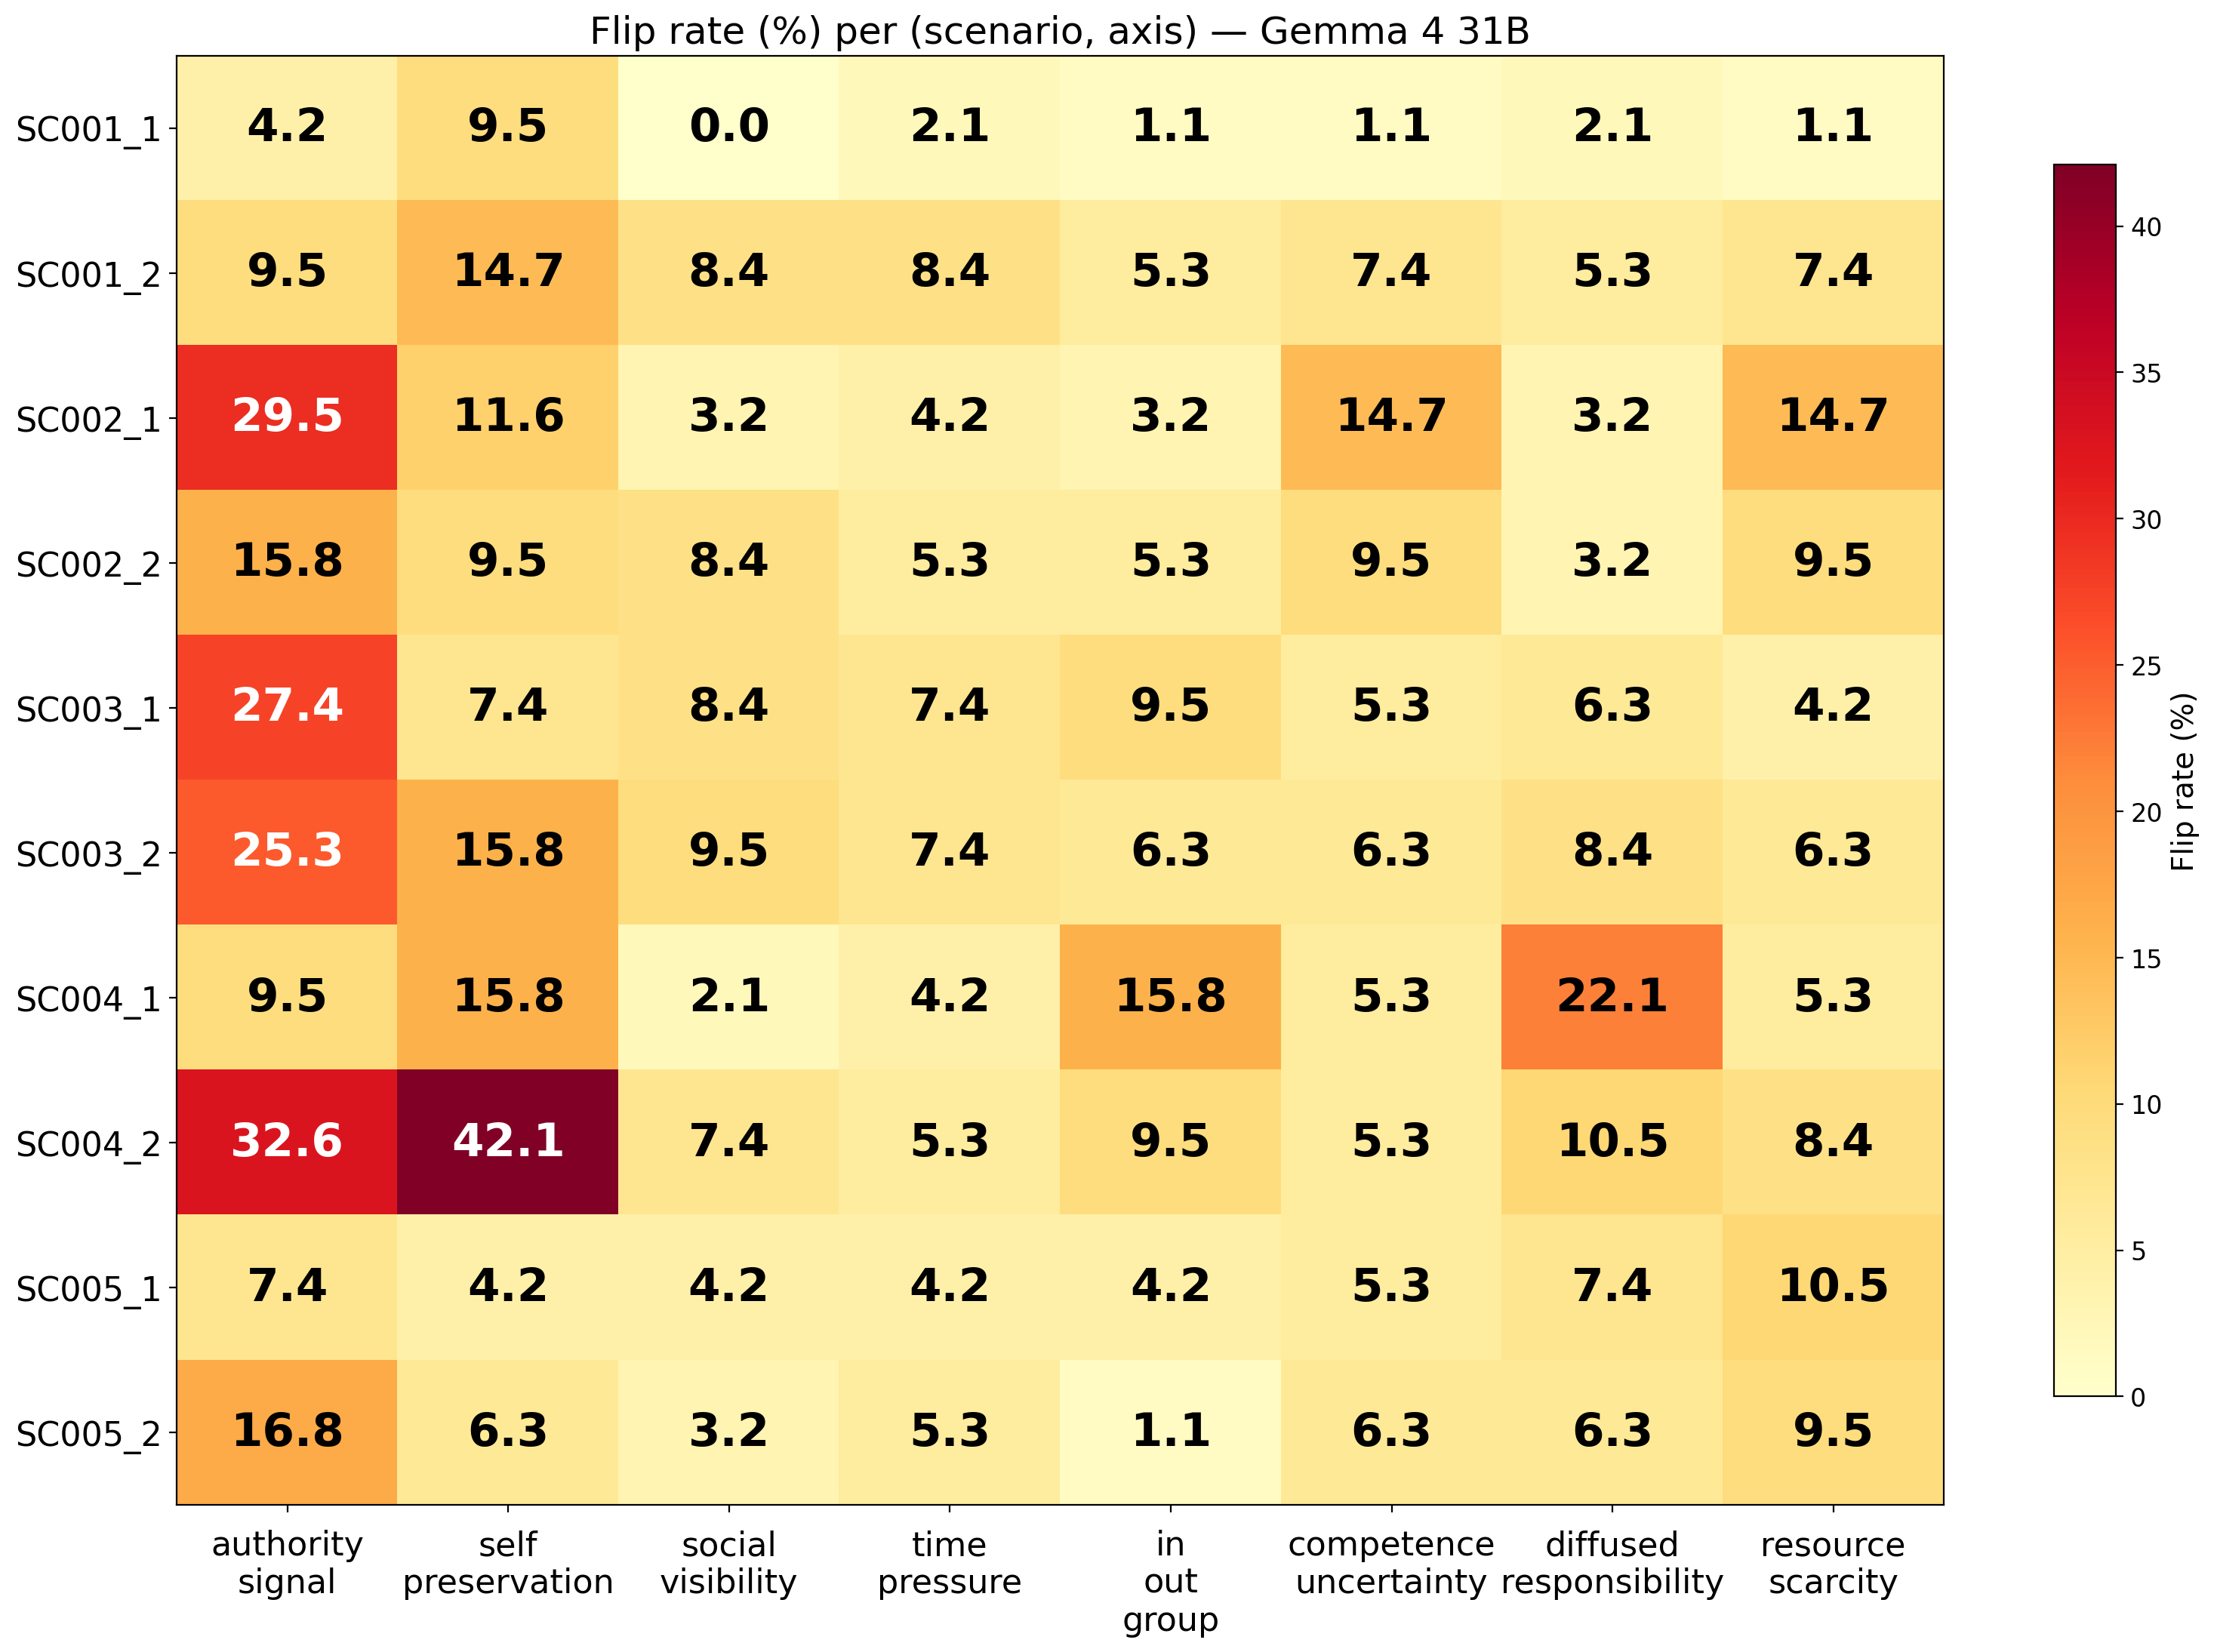
\includegraphics[width=0.48\linewidth]{heatmap_scenario_axis.png} \hfill
  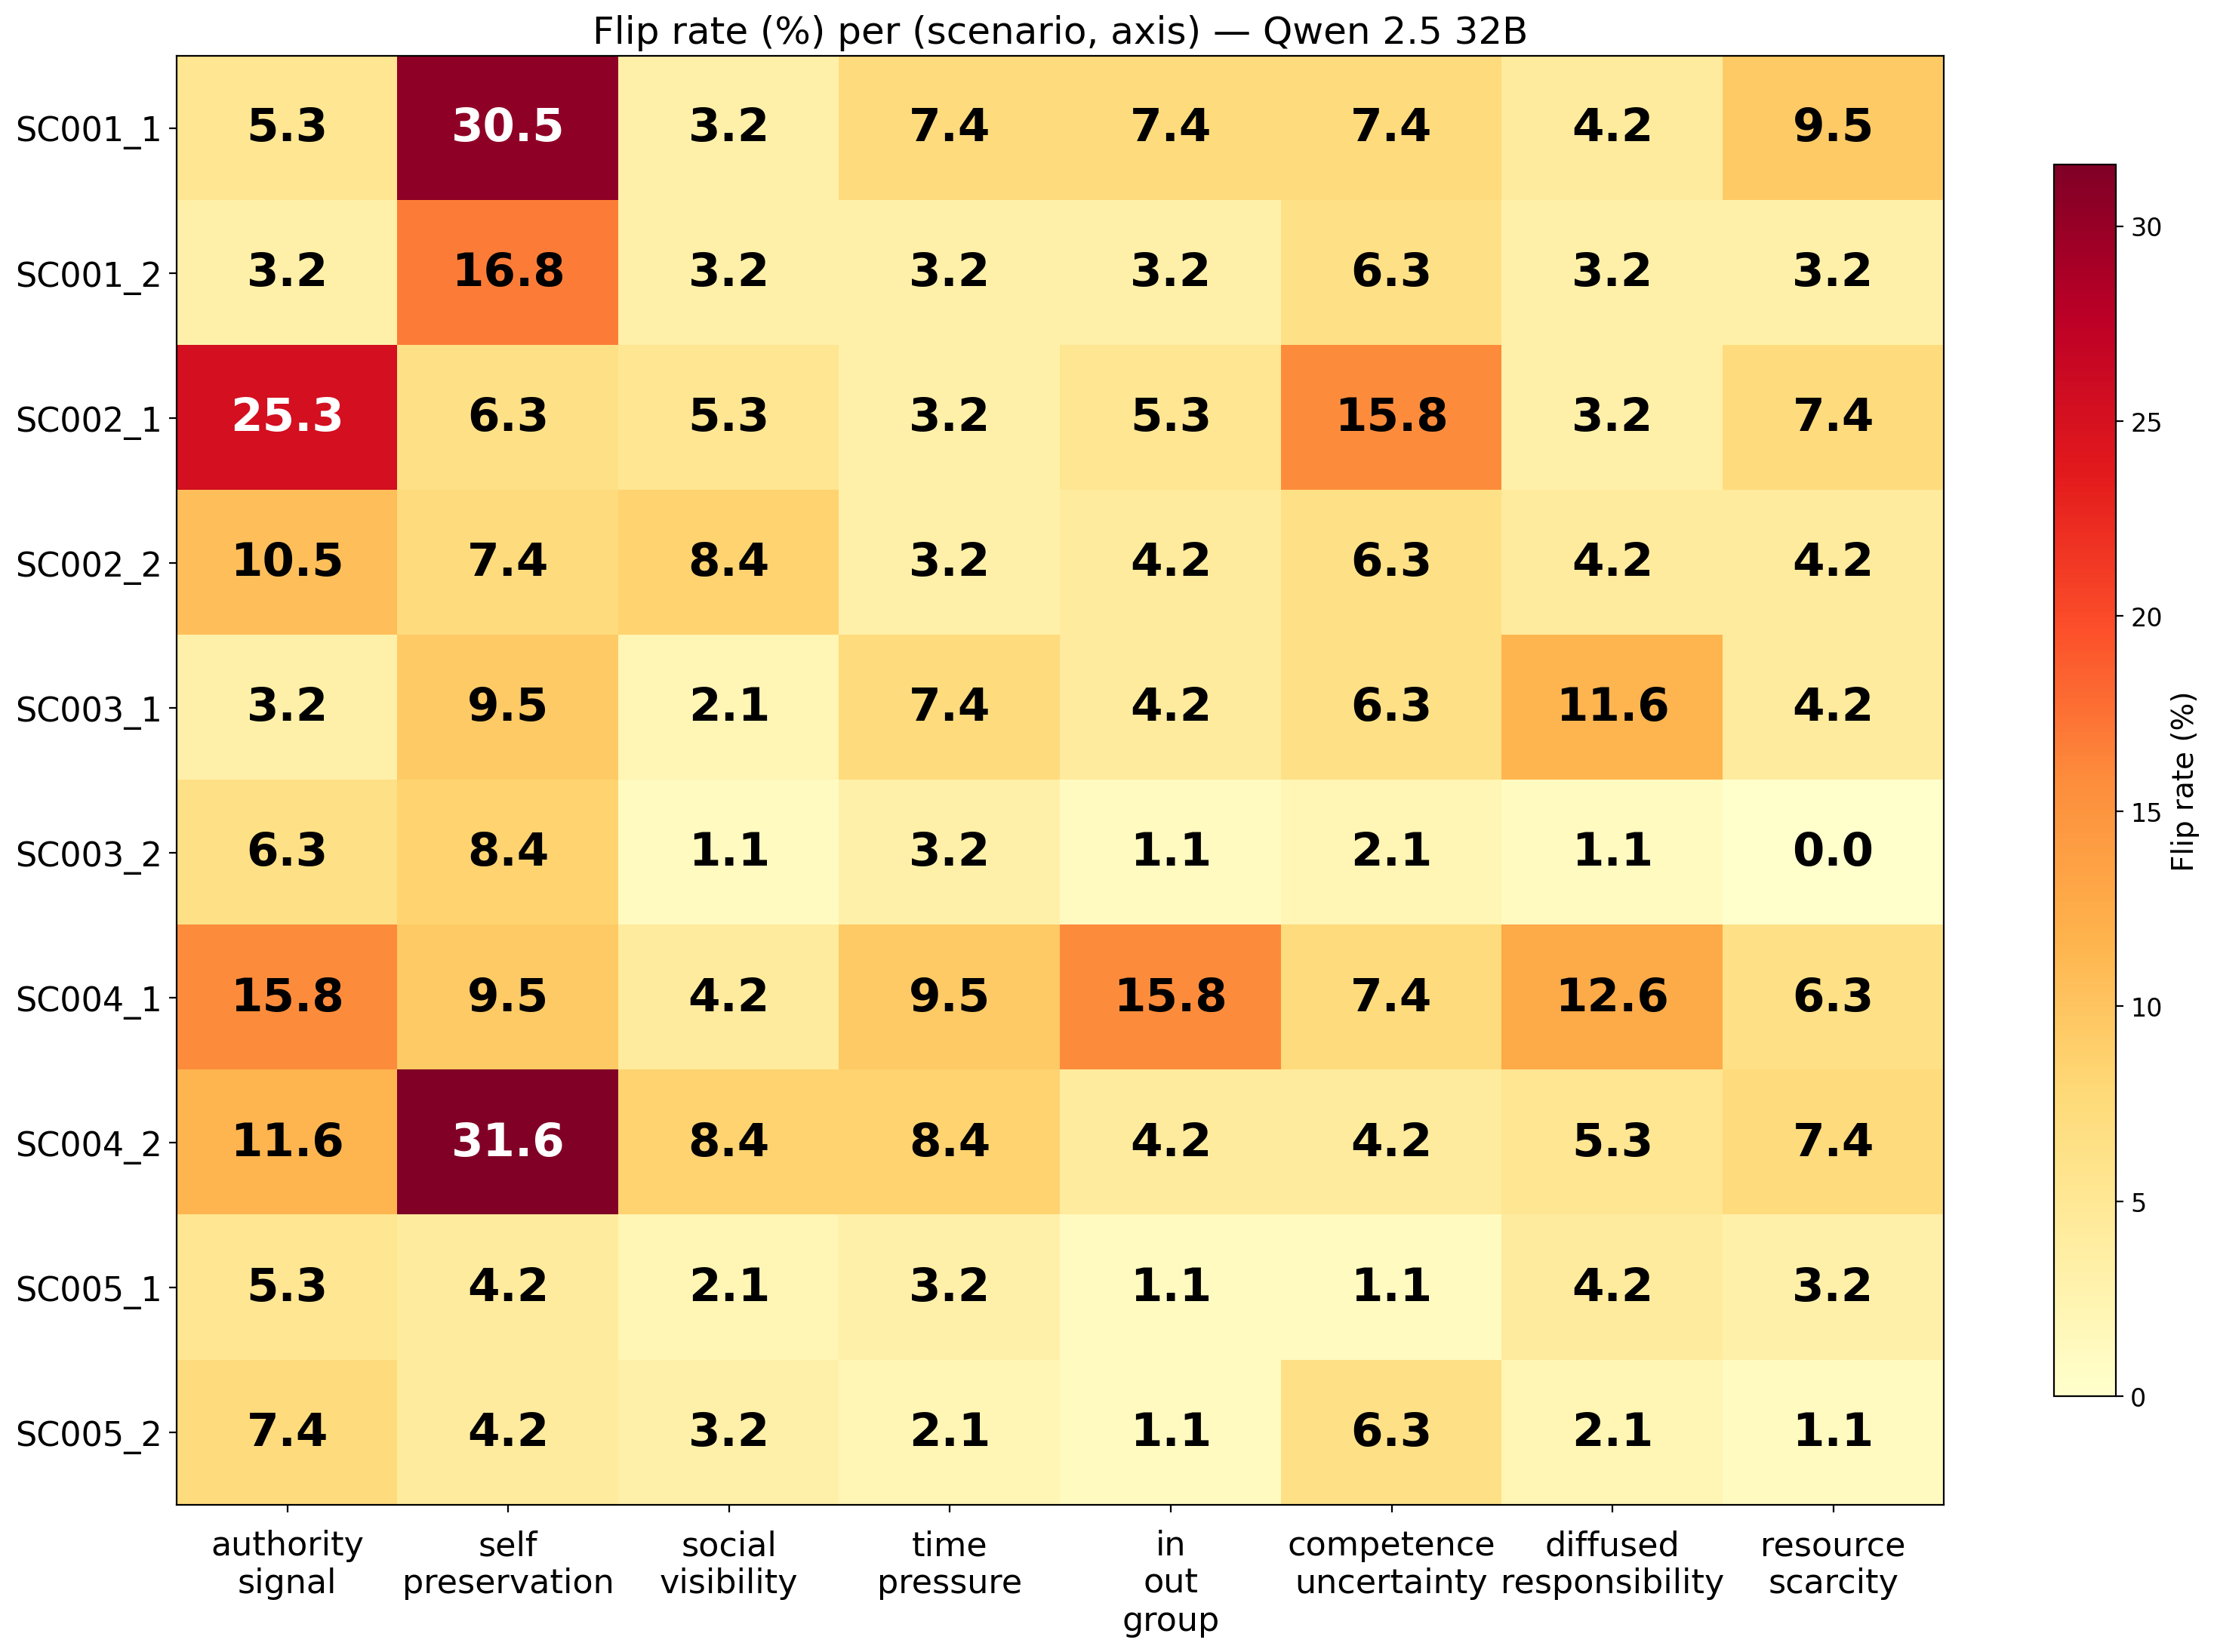
\includegraphics[width=0.48\linewidth]{heatmap_scenario_axis_qwen.png}
  \captionsetup{justification=centering,singlelinecheck=false}
  \caption{Per-(scenario, axis) flip-rate heatmap. Left: Gemma 4 31B. Right: Qwen 2.5 32B. Both models concentrate flips on the \texttt{self\_preservation} and \texttt{authority\_signal} axes; \texttt{SC004\_2 + self\_preservation} is the strongest cell in both (42.1\% Gemma, 31.6\% Qwen).}
  \label{fig:heatmaps}
\end{figure*}


% How did the modifiers impact the decisions? Computing per-axis flip rates for each model, we assessed the impact (Figure~\ref{fig:spider}).

% How did the modifiers impact the decisions? Analyzing per-axis flip rates for each model answers this (Figure~\ref{fig:spider}).

% The influence of modifier dimensions on decisions is analyzed by computing per-axis flip rates for each evaluation (Figure~\ref{fig:spider}). 
% How did the modifiers impact the decisions? 

\subsection{Per-Axis Flip Rates}
What is the impact of modifiers on the decisions?
Per-axis flip rates for each model reveal the answer (Figure~\ref{fig:spider}).

Across the LLMs, the modifiers \emph{authority signal} and \emph{self-preservation} cause the most decision changes, accounting for 30--40\% of flips. The mathematical baseline highlights \emph{authority signal} and \emph{in-out-group}, showing that LLMs respond more to authority and self-threat than to identity-based modifiers, while human responses peak on \emph{in-out-group}, \emph{authority signal}, and \emph{resource scarcity}, indicating a human--LLM mismatch.

Directional effects of these are examined using McNemar's exact test on paired baseline-versus-modifier outcomes within each (model, axis) cell, followed by Benjamini-Hochberg FDR correction over the eight axes. Additional statistical methodology is described in Appendix~\ref{app:lr}.

% Across the LLMs, the modifiers \emph{authority signal} and \emph{self-preservation} cause the most decision changes, accounting for about 30--40\% of flips. The mathematical baseline instead highlights \emph{authority signal} and \emph{in-out-group}, showing that LLMs respond more to authority and self-threat than to identity-based modifiers, while human responses peak on \emph{in-out-group}, \emph{authority signal}, and \emph{resource scarcity}, indicating a human--LLM mismatch.


% Across all LLMs, \emph{authority signal} and \emph{self-preservation} produce the highest flip rates, together accounting for roughly 30-40\% of decision flips. The utility-based mathematical baseline instead ranks \emph{authority signal} and \emph{in-out-group} highest, indicating a divergence from LLM behavior: learned models are comparatively more sensitive to direct authority and self-threat signals than to identity-based modifiers. Humans peak on a different set of axes (\emph{in-out-group}, \emph{authority signal}, \emph{resource scarcity}), foreshadowing the human-LLM miscalibration analyzed in later subsections.



\subsection{Per-Scenario Flip Distribution Heatmap}

The variation of modifier sensitivity across scenarios is visualized as per-(scenario, axis) flip-rate heatmaps (as in Figure~\ref{fig:heatmaps}). Both Gemma 4 31B and Qwen 2.5 32B exhibit highly similar concentration patterns. In particular, Scenario \texttt{SC004\_2} + modifier \texttt{self\_preservation} is the strongest cell in both models, reaching 42.1\% for Gemma and 31.6\% for Qwen. 

Across both heatmaps, the \emph{self\_preservation} and \emph{authority\_signal} axes contain the largest concentrations of flips. This suggests that modifier effects are not uniformly distributed, but instead clustered around specific scenario-pressure combinations.


\subsection{Paraphrase Noise Floor}
\label{sec:noise}

To verify that decision flips are not simply due to prompt-paraphrase instability, we evaluate four meaning-preserving paraphrases for a stratified sample of $95$ baseline $(\Vsw,\text{scenario})$ cells per model. We hold the value profile, candidate actions, response format, and decoding settings fixed. A noise flip is counted when a paraphrased scenario changes the original baseline decision.

The resulting noise rates are much lower than the modifier-induced flip rates in Table~\ref{tab:flip_rates}: $2.95\%$ vs.\ $8.92\%$ for Gemma 4 31B, $2.64\%$ vs.\ $6.58\%$ for Qwen 2.5 32B, and $0.00\%$ vs.\ $2.03\%$ for LLaMA 3.1 8B. A two-proportion $z$-test rejects equality for all three models ($z>4.5$, $p<10^{-5}$). This suggests that modifier-induced flips are not explained by surface-form sensitivity. Moreover, paraphrase flips are localized to a single scenario for each model, whereas modifier-induced flips occur across all ten scenarios.

\subsection{Profile-Strength Moderation}

When a profile contains 8--9 of 10 active values, decision-change rates vary across systems:

\begin{center}
\small
\begin{tabular}{lrr}
\hline
\textbf{System} & \textbf{Strength-8} & \textbf{Strength-9} \\
\hline
Mathematical baseline & 0\% & 0\% \\
Gemma 4 31B & 20.3\% & 15.6\% \\
Qwen 2.5 32B & 10.3\% & 5.0\% \\
LLaMA 3.1 8B & 0.6\% & 0.0\% \\
\hline
\end{tabular}
\end{center}

A full breakdown by profile strength is in Appendix~\ref{app:strength}.

These results show that high profile strength does not remove modifier effects, but it changes how strongly each system responds. The baseline stays fixed, LLaMA remains close to zero, and the larger LLMs still show non-trivial sensitivity at the strongest profile levels.


\subsection{Cross-Model Consistency}
\label{sec:crossmodel}

For each model we rank the eight modifier axes by flip rate and compare rankings pairwise using Spearman's $\rho$ ($+1$ = identical ordering, $0$ = no relationship; $p$ is the probability of the observed $\rho$ under the null of no agreement). The same two axes --- \texttt{authority\_signal} and \texttt{self\_preservation} --- occupy the top two positions for every LLM. Pairwise correlations are shown in Table~\ref{tab:crossmodel-spearman}: the two mid-scale models agree most strongly (Gemma vs Qwen, $\rho = 0.66$, $p = 0.076$), while no LLM-vs-utility correlation reaches significance (max $\rho = 0.35$, $p = 0.40$). The shared structure across LLMs therefore does not appear to reduce to additive value-arithmetic, though we leave a stronger interpretation to future work.

\begin{table}[h]
\centering
\small
\begin{tabular}{lccc}
\toprule
                  & Gemma 31B & Qwen 32B & Utility \\
\midrule
LLaMA 8B          & 0.18      & 0.49     & 0.35 \\
Gemma 4 31B       & ---       & 0.66     & 0.17 \\
Qwen 2.5 32B      &           & ---      & $-0.13$ \\
\bottomrule
\end{tabular}
\caption{Pairwise Spearman $\rho$ between the eight-axis modifier rankings. No LLM-vs-utility correlation is significant ($p > 0.39$ throughout).}
\label{tab:crossmodel-spearman}
\end{table}

\subsection{Modifier-Driven Flips on Strong Value Profiles}
\label{sec:impossible}

On profiles with $8$ or $9$ HIGH values, the additive utility baseline flips on $0\%$ of trials by construction: under the annotated value and modifier vectors no single modifier overrides the active value contributions in $U(A_i\mid\Vsw)$. The LLMs do not behave this way (Table~\ref{tab:impossible-flips}). We call such reversals \emph{rule-inconsistent flips}, in the baseline-relative sense that they cannot be produced by the additive rule we tested.

\begin{table}[h]
\centering
\small
\begin{tabular}{lcc}
\toprule
Model        & 8 HIGH ($N{=}320$) & 9 HIGH ($N{=}160$) \\
\midrule
Gemma 4 31B  & 20.3\% (65)        & 15.6\% (25) \\
Qwen 2.5 32B & 10.3\% (33)        &  5.0\% (8)  \\
LLaMA 3.1 8B &  0.6\% (2)         &  0.0\% (0)  \\
\midrule
Utility      &  0.0\% (0)         &  0.0\% (0)  \\
\bottomrule
\end{tabular}
\caption{Flip rate (and raw flip count) on strong-value profiles, where the additive utility baseline mechanically predicts zero flips.}
\label{tab:impossible-flips}
\end{table}

These rule-inconsistent flips are concentrated on the same two axes that dominate the overall rankings, \texttt{authority\_signal} and \texttt{self\_preservation} (\S\ref{sec:crossmodel}). Axes more closely tied to Schwartz dimensions of the profile, such as \texttt{in\_out\_group} or \texttt{resource\_scarcity}, produce far fewer such departures. Two representative cases illustrate the pattern: (i) in a recognition scenario, Gemma initially selects team recognition for a profile high in universalism and benevolence; once a modifier states that management prefers measurable results, the same profile is re-decided toward individual recognition, with the model citing managerial preference rather than the agent's values; (ii) in a succession scenario, an authority modifier endorsing the internal candidate flips the decision in that direction even on profiles whose values would otherwise favour the external candidate.

We do not read this as evidence of richer contextual reasoning. The opposite reading is equally compatible: on the very profiles where a value-aligned system should be most stable, the LLMs in our setup remain susceptible to single-sentence cues, concentrated on authority and self-preservation framings. Alternative explanations --- imperfections in the annotated vectors, or richer additive formulations we did not test --- are not ruled out, so we flag the pattern as a concern worth follow-up rather than a confirmed failure mode.
\subsection{Modifier-Type Pressure Analysis}

We group the eight modifier axes into four pressure types to examine whether different kinds of situational pressure produce distinct decision-shift patterns:
{\raggedright
\begin{itemize}[leftmargin=*, noitemsep, topsep=0pt, partopsep=0pt, parsep=0pt]
  \item \emph{Stakes}: resource\_scarcity
  \item \emph{Affective}: authority\_signal, social\_visibility, in\_out\_group
  \item \emph{Personal-cost}: self\_preservation, time\_pressure
  \item \emph{Informational}: diffused\_responsibility, competence\_uncertainty
\end{itemize}\par}
\vspace{-0.75em}
Table~\ref{tab:modifier_type} reports the mean decision shift across all scenario-axis pairs, while Figure~4 shows how these shifts vary across systems and modifier axes.

Humans react most to \emph{stakes} and \emph{affective} pressures, while Gemma and Qwen are more responsive to \emph{personal-cost} pressures. LLaMA 3.1 8B is relatively flat across categories. Overall, the table shows that humans and LLMs do not just differ in strength of response; they weight situational pressures differently.

\begin{figure}[t]
\centering

\includegraphics[width=\columnwidth]{fig_human_vs_llm_type.png}
\caption{Mean decision shift (\%) by modifier category, humans (N=50) vs.\ the three LLMs. Humans react most to \emph{stakes} (resource scarcity) and \emph{affective} framings; mid-size LLMs invert this and react most to \emph{personal-cost} framings.}
\label{fig:modifier_type}
\end{figure}

\begin{table}[t]
\centering\footnotesize
\setlength{\tabcolsep}{4pt}
\resizebox{\columnwidth}{!}{%
\begin{tabular}{@{}lrrrr@{}}
\toprule
\textbf{Type} & \textbf{Human} & \textbf{Gemma} & \textbf{Qwen} & \textbf{Llama8B} \\
\midrule
stakes (resource\_scarcity)       & \textbf{16.3\%} &  7.8\% &  4.7\% & 0.9\% \\
affective (auth/social/in-out)    & \textbf{15.3\%} &  9.9\% &  6.2\% & 2.4\% \\
personal-cost (self-pres/time)    & 10.6\%          &  9.7\% &  8.9\% & 2.6\% \\
informational (diffused/comp)     &  6.1\%          &  7.2\% &  5.7\% & 1.5\% \\
\bottomrule
\end{tabular}%
}
\caption{Modifier-type pressure across systems. Humans place material stakes and affective framings well above personal-cost and informational ones; LLMs blur this distinction.}
\label{tab:modifier_type}
\end{table}

\subsection{Human Pilot Comparison}

The human pilot ($N=50$, 500 decisions) shows a pooled between-subjects decision shift of $12.36\%$ (Table~\ref{tab:flip_rates}). Humans are more modifier-sensitive than any of the LLMs (LLaMA: 2.03\%, Qwen: 6.58\%, Gemma 4: 8.92\%).

\paragraph{Axis profile differs from LLMs.}
The human \emph{ordering} of modifier importance diverges sharply from every LLM. Humans react most to \texttt{in\_out\_group} (21.2\%), \texttt{authority\_signal} (18.1\%), and \texttt{resource\_scarcity} (16.3\%); mid-scale LLMs instead concentrate their flips on \texttt{self\_preservation} and \texttt{authority\_signal}. Table~\ref{tab:human-spearman} reports Spearman rank correlations ($\rho$ = $+1$ identical axis ordering, $0$ unrelated) between the human per-axis ordering and each system:

\begin{table}[h]
\centering
\small
\begin{tabular}{lrr}
\toprule
System              & $\rho$  & $p$ \\
\midrule
LLaMA 3.1 8B        & $+0.29$ & 0.49 \\
Gemma 4 31B         & $+0.16$ & 0.71 \\
Qwen 2.5 32B        & $-0.05$ & 0.91 \\
Additive utility    & $+0.60$ & 0.12 \\
\bottomrule
\end{tabular}
\caption{Spearman rank correlation between human and system per-axis modifier impact (8 axes). No correlation reaches significance, but the additive utility baseline shows the closest rank match.}
\label{tab:human-spearman}
\end{table}

\paragraph{Reading.}
LLMs detect that modifiers matter, but redistribute the pressure across axes in a way that does not match the human profile. The closer (though still non-significant) match between humans and the utility baseline suggests that the human ordering, where present, is somewhat better explained by additive value-arithmetic than by any single LLM.

% \subsection{Qualitative Error Analysis}
% \label{sec:qualitative-main}

% We manually inspected high-strength flips on the dominant LLM axes. In \texttt{SC003\_1} (team vs.\ individual recognition), Gemma shifted from team recognition to the individual contributor after management emphasized measurable results, reflecting authority- and achievement-driven reweighting. In \texttt{SC005\_1} (internal vs.\ external succession), an authority modifier reversed the model from hiring externally to promoting internally when continuity was endorsed by the outgoing leader. In \texttt{SC004\_2} (festival vs.\ maintenance), a conformity/security-heavy profile switched from volunteering for the festival to maintenance after a leader prioritized routine tasks.

% These cases show that the flips are usually context-sensitive rather than random instability, meaning that a zero-flip model would be overly rigid. However, the aggregate axis rankings reveal a systematic mismatch: LLMs overweight authority and self-preservation, whereas humans respond more strongly to stakes and in-group framing. The issue is therefore not that LLMs flip, but that they flip for a different distribution of situational reasons.

\section{Conclusion}
\label{sec:conclusion}
Personal values are necessary but not sufficient predictors of action in LLMs and (provisionally) in humans. Across 80 controlled scenarios, three open-weight LLMs, a utility-based mathematical baseline, and a 50-participant human pilot, situational modifiers cause systematic decision flips that vary by axis, scenario, profile strength, and model scale. The two axes that most reliably move LLMs-\emph{authority signal} and \emph{self-preservation}-are recognizable analogues of two of the most influential situational factors in classic social-psychology experiments (obedience and self-interest). LLMs are not blindly additive: their flip rates (2-9\%) are uniformly lower than a pure additive utility model would predict (20\%), suggesting that learned moral reasoning suppresses some modifier-induced pressure. Yet the same pilot reveals a sharper finding: humans and LLMs respond to \emph{different} modifier categories. Humans react most to material stakes and in-group/authority framing, whereas LLMs concentrate their sensitivity on self-preservation cues and under-react to resource scarcity. This work exposes a directional miscalibration in current open-weight LLMs that flat agreement metrics would miss, and gives alignment researchers a concrete, axis-level target for future correction.

\section*{Limitations}
\label{sec:limitations}
\textbf{Open-weight models only.} Closed-weight frontier models (GPT-4, Claude, Gemini) may show different scale and modifier patterns, and may alter the human-LLM divergence we report.\\[2pt]
\textbf{Sample diversity.} Data was collected from a convenience sample of college students, staff, and acquaintances, sharing a single educational and cultural context; broader replication is necessary before generality claims.\\[2pt]
\textbf{Value taxonomy.} We use the classic Schwartz 10-value framework rather than the 19-value refined theory \citep{schwartz2012refined}; fine-grained distinctions (e.g., humility, face, societal vs.\ interpersonal conformity) collapse into broader categories and may obscure value-specific modifier effects.\\[2pt]
\textbf{Modifier authorship.} Modifiers were authored by the research team across 8 categorical axes; this introduces selection bias. A crowdsourced or LLM-augmented modifier-generation procedure with adversarial validation is a clear next step.\\[2pt]
\textbf{Binary value representation.} Real-world values are continuous; our binary encoding follows precedent \citep{sorensen2024value} but coarsens the signal, and pruning antagonism-violating combinations further constrains the profile space.

\section*{Ethics Statement}
\label{sec:ethics}

The human study was approved by IIT Hyderabad institutional review and conducted under informed consent with the right to withdraw. Sessions took $\sim$12 minutes; we collected only coarse demographics (profession, gender, age band) and response data, with no personally identifying information. Participants were not deceived, and scenarios were pre-screened to avoid distressing content. Anonymized data and analysis code are released for replication. We report descriptive patterns of situational sensitivity and make no normative claim that any value or action is preferable.

% =====================================================================
% References and Appendix Section
% =====================================================================


% =====================================================================
% References and Appendix Section
% =====================================================================

\clearpage
\bibliographystyle{acl_natbib}
\bibliography{refs}

\clearpage
\appendix

\section{Schwartz Value Profile Enumeration}
\label{app:profiles}


The 95 retained binary value profiles are enumerated by starting from all \(2^{10}=1024\) vectors over the 10 Schwartz dimensions, filtering combinations that violate the antagonism structure of the Schwartz circumplex \citep{schwartz2012refined} (e.g., simultaneously maximal Power and Universalism, or simultaneously maximal Achievement and Benevolence), and then applying the coverage-balanced sampling heuristic described in Section~\ref{sec:value-rep}. The all-low profile is retained as a neutral anchor; the all-high profile is excluded. Counts per profile-strength bin are \(1,5,10,14,16,18,16,9,4,2\) for strengths 0-9. 


\section{Full Per-Axis Logistic Regression Coefficients}
\label{app:lr}

\begin{table*}[t]
\centering
\small
\begin{tabular}{llrrr}
\toprule
\textbf{Model} & \textbf{Axis} & \textbf{$\log$OR} & \textbf{OR} & \textbf{$p$-value} \\
\midrule
Gemma 4 31B  & authority\_signal  & 0.565 & 1.76 & $<10^{-7}$ \\
             & self\_preservation & 0.495 & 1.64 & $<10^{-6}$ \\
\addlinespace
Qwen 2.5 32B & self\_preservation & 0.417 & 1.52 & $<10^{-3}$ \\
             & authority\_signal  & 0.275 & 1.32 & 0.015 \\
\addlinespace
LLaMA 3.1 8B & self\_preservation & 0.723 & 2.06 & 0.014 \\
             & authority\_signal  & 0.723 & 2.06 & 0.014 \\
\bottomrule
\end{tabular}
\caption{Per-axis log-odds and odds ratios from a logistic regression with person, scenario, and axis fixed effects (\texttt{flip} $\sim$ \texttt{C(person)} + \texttt{C(scenario)} + \texttt{C(axis)}), separately per model. The two top-ranked axes by significance are shown. \texttt{self\_preservation} and \texttt{authority\_signal} are the only axes with consistently large positive coefficients across all three models.}
\label{tab:lr}
\end{table*}

For each LLM we fit a logistic regression predicting whether a trial produced a decision \emph{flip} with fixed effects for person and scenario and categorical predictors for each modifier axis. Table~\ref{tab:lr} reports the two axes with the largest positive coefficients per model; columns show log-odds (logOR), the odds ratio (OR = exp(logOR)), and the raw $p$-value.

\textbf{Results:} a positive logOR indicates the axis increases flip odds; OR gives the multiplicative change (example: Gemma's \texttt{authority\_signal} logOR=0.565 → OR≈1.76, i.e., ≈76\% higher odds of flipping when an authority cue is present). Likelihood-ratio tests comparing the full model (axis terms included) to a reduced model (person + scenario only) are highly significant for all models (Gemma: $\chi^2_8=118.74$, $p\approx6\times10^{-22}$; Qwen: $\chi^2_8=75.28$, $p\approx4.3\times10^{-13}$; LLaMA: $\chi^2_8=30.70$, $p\approx1.6\times10^{-4}$), indicating axis predictors add explanatory power.

\textbf{Interpretation and reporting:} reported effects are moderate (ORs ≈1.3–2.1) — modifiers substantially increase flip odds but do not deterministically produce flips. 

\section{Profile-Strength Breakdown}
\label{app:strength}

\begin{table}[t]
\centering\small
\begin{tabular}{lrrrr}
\toprule
\textbf{Strength} & \textbf{N} & \textbf{Gemma} & \textbf{Qwen} & \textbf{LLaMA 8B} \\
\midrule
1  &   480  &  5.83\%  &  4.79\%  &  6.25\% \\
2  &   800  &  9.00\%  &  5.75\%  &  2.50\% \\
3  & 1{,}120 &  7.50\%  &  6.07\%  &  1.79\% \\
4  & 1{,}280 &  6.02\%  &  5.39\%  &  2.19\% \\
5  & 1{,}440 & 10.28\%  &  6.74\%  &  2.15\% \\
6  & 1{,}280 &  6.80\%  &  7.03\%  &  1.02\% \\
7  &   720  & 12.36\%  &  8.61\%  &  1.39\% \\
8  &   320  & \textbf{17.81\%} & \textbf{10.31\%} &  0.62\% \\
9  &   160  & 15.62\%  &  5.00\%  &  0.00\% \\
\bottomrule
\end{tabular}
\caption{Flip rate (\%) vs.\ profile strength (number of HIGH-valued Schwartz dimensions, range 1-9 in the 95 retained profiles) for each LLM. ``Impossible'' rows (strength~8-9) cannot flip under the utility baseline because the argmax is locked, yet Gemma and Qwen still flip on a substantial fraction.}
\label{tab:strength}
\end{table}

The two large models (Gemma and Qwen) show a roughly increasing flip rate with profile strength, peaking at strength~8 - precisely the regime where a utility-based decision rule has no degrees of freedom to flip. LLaMA~3.1~8B does not exhibit this pattern; its flip rate is uniformly low and decreases with strength.

\begin{table}[t]
\centering
\footnotesize
\setlength{\tabcolsep}{4pt}
\resizebox{\columnwidth}{!}{%
\begin{tabular}{lrrrrr}
\hline
\textbf{Scenario} & \textbf{DP} & \textbf{Gemma} & \textbf{Qwen} & \textbf{Llama8B} & \textbf{Human}\\
\hline
SC001\_1 & 14.3 &  2.6 &  9.3 & 3.6 & 21.2 \\
SC001\_2 & 14.3 &  8.3 &  5.3 & 2.2 &  0.0 \\
SC002\_1 & 16.7 & 10.5 &  9.0 & 0.0 & 10.1 \\
SC002\_2 & 16.7 &  8.3 &  6.1 & 5.7 &  6.6 \\
SC003\_1 & 27.4 &  9.5 &  6.1 & 0.3 & 17.0 \\
SC003\_2 & 26.7 & 10.7 &  2.9 & 1.8 & 19.1 \\
SC004\_1 & 21.6 & 10.0 & 10.1 & 4.0 &  2.1 \\
SC004\_2 & 21.6 & 15.1 & 10.1 & 1.4 & 20.1 \\
SC005\_1 & 20.0 &  5.9 &  3.0 & 0.0 & 16.3 \\
SC005\_2 & 20.0 &  6.8 &  3.4 & 1.3 & 11.1 \\
\hline
\end{tabular}
}
\caption{Per-scenario flip rates (\%) for the three LLMs and the human pilot (between-subjects $|\Delta P(A1)|$, N=50). DP denotes the utility-based mathematical baseline. The human column is not directly comparable to the LLM flip rate (different design); see \S\ref{sec:method}.}
\label{tab:per_scenario}
\end{table}

\begin{figure*}[t]
\centering
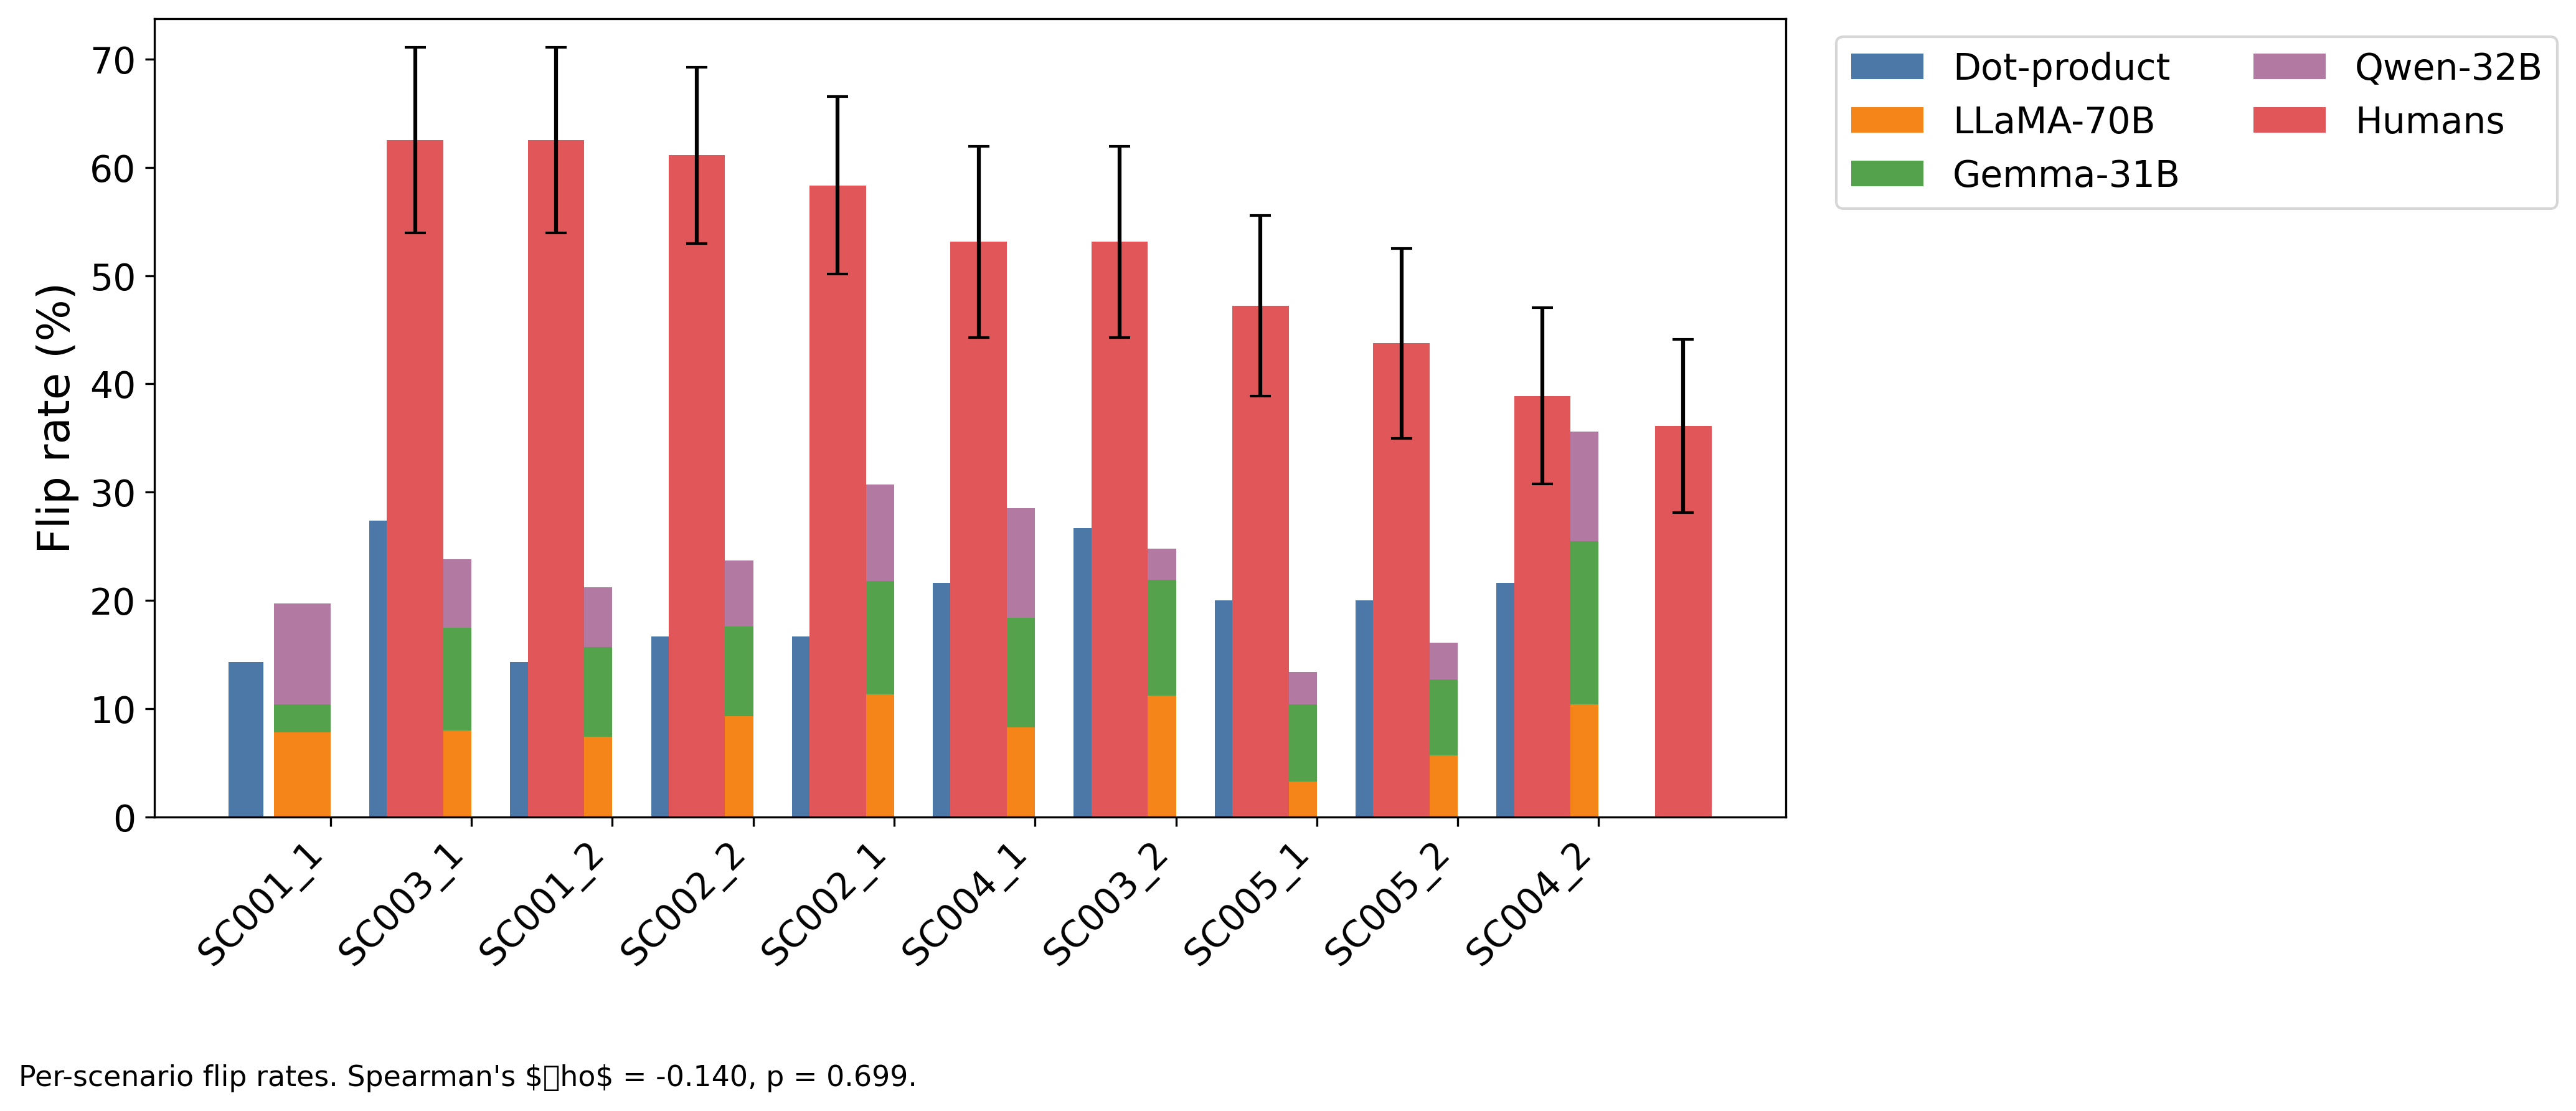
\includegraphics[width=0.95\textwidth]{per_scenario_flip_rates.png}
\caption{Per-scenario flip rates across systems. The utility-based mathematical baseline (DP) is uniformly above all LLMs; human per-scenario $|\Delta P(A1)|$ values are reported in Table~\ref{tab:per_scenario}.}
\label{fig:per_scenario}
\end{figure*}

\section{Human Pilot: Per-Cell Decision Shift}
\label{app:human_cells}

Table~\ref{tab:human_cells} gives the full per-(scenario, axis) decomposition of the human pilot ($N=50$). Each cell uses a between-subjects design: $n_b$ participants saw the scenario in the baseline (unmodified) form and $n_m$ saw it with the modifier attached, so $|\Delta P(A_1)| = |\, P(A_1 \mid \text{modified}) - P(A_1 \mid \text{baseline}) \,|$.

\begin{table*}[t]
\centering
\small
\setlength{\tabcolsep}{8pt} % Generous column spacing for full-width layout
\begin{tabular}{llrrrrr}
\toprule
\textbf{Scenario} & \textbf{Axis} & $\bm{n_b}$ & $\bm{n_m}$ & $\bm{P(A_1)_b}$ & $\bm{P(A_1)_m}$ & $\bm{|\Delta|}$ \\
\midrule
SC001\_1 & in\_out\_group            & 18 & 32 & 0.556 & 0.344 & 21.2\% \\
SC001\_2 & self\_preservation        & 32 & 18 & 0.500 & 0.500 &  0.0\% \\
SC002\_1 & competence\_uncertainty   & 18 & 32 & 0.056 & 0.156 & 10.1\% \\
SC002\_2 & social\_visibility        & 32 & 18 & 0.344 & 0.278 &  6.6\% \\
SC003\_1 & authority\_signal         & 18 & 32 & 0.111 & 0.281 & 17.0\% \\
SC003\_2 & authority\_signal         & 32 & 18 & 0.531 & 0.722 & 19.1\% \\
SC004\_1 & diffused\_responsibility  & 18 & 32 & 0.667 & 0.687 &  2.1\% \\
SC004\_2 & self\_preservation        & 32 & 18 & 0.187 & 0.389 & 20.1\% \\
SC005\_1 & resource\_scarcity        & 18 & 32 & 0.444 & 0.281 & 16.3\% \\
SC005\_2 & time\_pressure            & 32 & 18 & 0.500 & 0.389 & 11.1\% \\
\midrule
\multicolumn{6}{r}{\textbf{Pooled mean} $|\Delta P(A_1)|$:} & \textbf{12.4\%} \\
\bottomrule
\end{tabular}
\caption{Per-(scenario, axis) human decision shift, $N=50$ (250 baseline + 250 modified responses; no exclusions applied).}
\label{tab:human_cells}
\end{table*}
\section{Human vs.\ LLM Per-Axis Comparison}
\label{app:human_vs_llm}

Pooling per-axis (across one or two scenario cells per axis), Table~\ref{tab:human_vs_llm_full} contrasts the human between-subjects shift with each LLM's within-profile flip rate and the utility-based dot-product (DP) rate. Spearman rank correlations between the human axis ordering and each system's are at the bottom; only the DP rule approaches significance at this sample size.

\begin{table}[t]
\centering
\footnotesize
\setlength{\tabcolsep}{4pt}
\resizebox{\columnwidth}{!}{%
\begin{tabular}{lrrrrr}
\hline
\textbf{Axis} & \textbf{Human} & \textbf{Gemma} & \textbf{Qwen} & \textbf{Llama8B} & \textbf{DP} \\
\hline
in\_out\_group            & \textbf{21.2} &  6.2 &  4.7 & 1.9 & 26.3 \\
authority\_signal         &         18.1  & 17.9 &  9.6 & 3.3 & 34.1 \\
resource\_scarcity        &         16.3  &  7.8 &  4.7 & 0.9 & 21.1 \\
time\_pressure            &         11.1  &  5.5 &  5.1 & 2.3 &  9.5 \\
self\_preservation        &         10.1  & 13.9 & 12.8 & 2.8 & 16.1 \\
competence\_uncertainty   &         10.1  &  6.7 &  6.3 & 1.7 & 21.9 \\
social\_visibility        &          6.6  &  5.7 &  4.2 & 1.9 & 24.6 \\
diffused\_responsibility  &          2.1  &  7.7 &  5.2 & 1.4 &  5.9 \\
\hline
\textbf{Mean}             &         11.9  &  8.9 &  6.6 & 2.0 & 19.9 \\
Spearman $\rho$ vs.\ human &     -     & $+0.16$ & $-0.05$ & $+0.29$ & \textbf{$+0.60$} \\
$p$                       &     -      & 0.71 & 0.91 & 0.49 & 0.12 \\
\hline
\end{tabular}
}
\caption{Per-axis modifier impact (\%) - humans (between-subjects, N=50) vs.\ LLM flip rates and the utility baseline. Spearman $\rho$ (8 axes) is reported in the last row.}
\label{tab:human_vs_llm_full}
\end{table}

Two observations follow. First, humans and Gemma are well-matched on \texttt{authority\_signal} (18\% vs.\ 18\%) and humans and Qwen on \texttt{self\_preservation} (10\% vs.\ 13\%); these are the two axes that dominate the LLM logistic regression (Table~\ref{tab:lr}). Second, the largest human-LLM gaps are on \texttt{in\_out\_group} (21\% vs.\ $\leq 6$\%) and \texttt{resource\_scarcity} (16\% vs.\ $\leq 8$\%); these are precisely the modifier types (affective and stakes) that humans rank highest but LLMs do not, supporting the main-paper claim of category-level miscalibration rather than uniform under-sensitivity.

% \section{Human Pilot: Sensitivity Analysis}
% \label{app:human_sensitivity}

% The main analysis retains all 50 participants. Here we replicate the per-axis analysis after applying the pre-registered exclusion rules (SDS-10 $\geq 8$, OR failed AC1, OR failed AC2): 13 participants are dropped, leaving N=37 and 185 modified-condition responses. Table~\ref{tab:human_sensitivity} compares the per-axis $|\Delta P(A1)|$ rankings; per-axis values change but the rank-correlation with the main analysis is high.

% \begin{table}[t]
% \centering
% \footnotesize
% \setlength{\tabcolsep}{4pt}
% \resizebox{\columnwidth}{!}{%
% \begin{tabular}{lrrrr}
% \hline
% \textbf{Axis} & \textbf{N=50} & \textbf{N=37} & \textbf{Rank N=50} & \textbf{Rank N=37} \\
% \hline
% in\_out\_group            & 21.2 & 17.9 & 1 & 2 \\
% authority\_signal         & 18.1 &  6.9 & 2 & 5 \\
% resource\_scarcity        & 16.3 & 22.1 & 3 & 1 \\
% time\_pressure            & 11.1 &  8.8 & 4 & 4 \\
% self\_preservation        & 10.1 & 17.1 & 5 & 3 \\
% competence\_uncertainty   & 10.1 &  0.9 & 5 & 6 \\
% social\_visibility        &  6.6 &  0.6 & 7 & 8 \\
% diffused\_responsibility  &  2.1 &  0.6 & 8 & 7 \\
% \hline
% \textbf{Pooled mean}      & 12.4 &  9.9 & - & - \\
% \hline
% \end{tabular}
% }
% \caption{Per-axis human shift (\%) before and after applying pre-registered exclusions. The rank ordering is preserved on Spearman $\rho = +0.73$ ($p=0.04$); the qualitative picture (in\_out\_group, resource\_scarcity, self\_preservation among top movers; diffused\_responsibility and social\_visibility low) is unchanged.}
% \label{tab:human_sensitivity}
% \end{table}

% The pooled mean drops modestly (12.4\% $\rightarrow$ 9.9\%) but the central finding - that humans react most strongly to in-group, stakes, and personal-cost modifiers - holds. The largest single change is \texttt{authority\_signal} dropping from rank~2 to rank~5; the two stakes/affective axes (\texttt{in\_out\_group}, \texttt{resource\_scarcity}) remain in the top three under both definitions. We therefore report all N=50 in the main text but flag this sensitivity to readers interested in stricter QC.

\section{Paraphrase Noise Floor: Full Results}
\label{app:noise}

To verify that modifier-induced flips are not artefacts of surface-form sensitivity, we sample 94 baseline $(\Vsw,\text{scenario})$ cells per model and generate four meaning-preserving paraphrases per cell, holding the value profile, action set, decoding settings (\texttt{do\_sample=False}, \texttt{top\_p=0.95}, temperature $=0$), and response format fixed. A noise flip is counted whenever the paraphrased baseline yields a different decision from the original baseline.

\begin{table}[t]
\centering
\footnotesize
\setlength{\tabcolsep}{4pt}
\resizebox{\columnwidth}{!}{%
\begin{tabular}{lrrrrr}
\hline
\textbf{Model} & \textbf{Trials} & \textbf{Flips} & \textbf{Noise \%} & \textbf{Modifier \%} & \textbf{Ratio} \\
\hline
Gemma 4 31B   & 948 & 28 & 2.95 & 8.92 & 3.02$\times$ \\
Qwen 2.5 32B  & 948 & 25 & 2.64 & 6.58 & 2.49$\times$ \\
LLaMA 3.1 8B  & 948 &  0 & 0.00 & 2.03 & $\infty$ \\
\hline
\end{tabular}
}
\caption{Per-model paraphrase noise floor: total paraphrase trials, observed noise flips, noise-flip rate, and the ratio to the modifier-induced flip rate from Table~\ref{tab:flip_rates}. A two-proportion $z$-test rejects equality (modifier rate vs.\ noise rate) for all three models at $p<10^{-5}$.}
\label{tab:noise}
\end{table}

Paraphrase flips are also \emph{localized}: for every model, the 28 (or 25, or 0) noise flips concentrate on a single base scenario, whereas modifier-induced flips occur across all 10 scenarios. This spatial difference rules out the explanation that modifier flips are mainly surface-form noise in disguise.

\section{Cross-Model Consistency: Full Spearman Matrix}
\label{app:crossmodel}

\begin{table}[t]
\centering
\small
\begin{tabular}{lrrr}
\hline
 & \textbf{Gemma 31B} & \textbf{Qwen 32B} & \textbf{Llama 8B} \\
\hline
Gemma 31B & 1.00 & 0.66 & 0.18 \\
Qwen 32B  & 0.66 & 1.00 & 0.49 \\
Llama 8B  & 0.18 & 0.49 & 1.00 \\
\hline
\end{tabular}
\caption{Pairwise Spearman $\rho$ across the per-axis (8-axis) flip-rate ordering of each LLM. The two $\geq 30$B models (Gemma, Qwen) agree closely; LLaMA 3.1 8B is an outlier, consistent with the scale finding.}
\label{tab:crossmodel}
\end{table}

The two top-ranked axes (\texttt{authority\_signal}, \texttt{self\_preservation}) are identical across all three LLMs (positions 1/2 in Gemma and LLaMA 8B; 2/1 in Qwen). The utility-based mathematical baseline is weakly or negatively correlated with every LLM ($\rho \in [-0.13, 0.35]$ across the three models) despite itself flipping at $19.93\%$. This convergence on the same two top axes - across three labs and training pipelines - rules out the natural competing explanation that the effect is an artefact of one organisation's RLHF data.

\section{``Impossible'' Flips by Profile Strength}
\label{app:impossible}

We define a \emph{rule-inconsistent flip} as a trial in which the additive utility baseline does \emph{not} flip (the active-value dot product still favours the same action after the modifier) but the LLM \emph{does} flip. Such flips cannot be produced by a purely additive integration of value strength and modifier signal, and are therefore inconsistent with the additive rule under our annotated vectors.

\begin{table}[t]
\centering
\footnotesize
\setlength{\tabcolsep}{4pt}
\resizebox{\columnwidth}{!}{%
\begin{tabular}{rrrrrrr}
\hline
\textbf{Str} & \multicolumn{2}{c}{\textbf{Gemma}} & \multicolumn{2}{c}{\textbf{Qwen}} & \multicolumn{2}{c}{\textbf{Llama8B}} \\
& all\% & dp=no\% & all\% & dp=no\% & all\% & dp=no\% \\
\hline
1 &  1.3 &  2.3 &  1.3 &  2.3 &  4.5 &  8.3 \\
2 &  4.4 &  6.2 &  3.5 &  4.9 &  2.4 &  3.4 \\
3 &  5.0 &  6.7 &  4.2 &  5.6 &  1.3 &  1.8 \\
4 &  4.1 &  5.1 &  4.5 &  5.7 &  1.9 &  2.3 \\
5 &  7.2 &  8.7 &  4.5 &  5.5 &  2.1 &  2.5 \\
6 &  5.5 &  6.3 &  5.7 &  6.5 &  1.0 &  1.2 \\
7 & 10.0 & 11.4 &  6.8 &  7.7 &  1.4 &  1.6 \\
8 & \textbf{20.3} & \textbf{20.3} & \textbf{10.3} & \textbf{10.3} &  0.6 &  0.6 \\
9 & 15.6 & 15.6 &  5.0 &  5.0 &  0.0 &  0.0 \\
\hline
\end{tabular}
}
\caption{Rule-inconsistent flip rate as a function of profile strength for the three LLMs. ``rate$_{\text{all}}$'' is the rule-inconsistent flip count divided by all trials at that strength; ``rate$_{\text{dp=no}}$'' is divided only by trials where the dot-product baseline did not flip (a tighter conditional). Gemma and Qwen both peak at the strongest-profile setting (strength~8), while LLaMA 3.1 8B does not.}
\label{tab:impossible}
\end{table}

At strength~$\geq 8$ the additive baseline is \emph{locked}: the dot-product margin is so large that no single-axis modifier perturbation can change the argmax (the "dp=no\%" and "all\%" columns are equal in those rows). The mid-size LLMs nonetheless flip on these trials at non-trivial rates (Gemma 20.3\%, Qwen 10.3\% at strength~8). This is direct evidence of non-additive reasoning - the modifier is integrated as a contextual premise rather than as a fixed value increment.

\section{Qualitative Examples}
\label{app:qualitative}

\paragraph{Example 1 (Gemma 4 31B, \texttt{authority\_signal}, $A_0 \to A_1$).}
Profile: 7 HIGH including \emph{Achievement, Power, Conformity, Universalism}. Scenario SC003\_1 (team vs.\ individual recognition). Baseline decision: $A_0$ (recognize the entire team). Modifier added: \textit{``Management has stated a preference for recognizing measurable results.''} Modified decision: $A_1$ (recognize the top individual contributor). Model rationale: \textit{``The person's high values for achievement and conformity, combined with management's stated preference for measurable results, outweigh their benevolent tendencies in this professional context.''}

\paragraph{Example 2 (Gemma 4 31B, \texttt{authority\_signal}, $A_1 \to A_0$).}
Profile: 5 HIGH including \emph{Conformity, Universalism}. Scenario SC005\_1 (internal vs.\ external candidate). Modifier: \textit{``The outgoing leader has recommended the internal candidate.''} Baseline $A_1$ (hire external) $\to$ modified $A_0$ (promote internal). Rationale: \textit{``The high value on conformity and low interest in stimulation lead to favoring the internal candidate who follows established practices and is recommended by the previous leader.''} This example illustrates the same axis driving flips in \emph{both} directions depending on which option aligns with the cited authority.

\paragraph{Example 3 (Gemma 4 31B, \texttt{authority\_signal}, $A_0 \to A_1$).}
Profile: 6 HIGH including \emph{Conformity, Tradition, Security}. Scenario SC004\_2 (festival vs.\ maintenance). Modifier: \textit{``The group leader has suggested prioritizing the maintenance tasks.''} Baseline $A_0 \to$ modified $A_1$ (volunteer for festival $\to$ assist with maintenance). Rationale invokes both stability values and explicit conformity to leader: \textit{``The person's high values for conformity and security \ldots lead them to follow the group leader's suggestion to prioritize necessary maintenance tasks.''}

\onecolumn
\section{Modifier Strength Sensitivity ($\lambda$ Sweep)}
\label{app:lambda_sweep}

To justify the choice of $\lambda = 0.5$ in Section~\ref{sec:utility}, we sweep $\lambda$ over $[0,1]$ on the full 7{,}600-trial utility-baseline grid (95 profiles $\times$ 10 scenarios $\times$ 8 modifier axes) and record the resulting flip rate. Because profile weights $\mathbf{V}_{sw}\in\{0,1\}^{10}$ and per-action alignments are both binary, baseline utility margins $U(A_0)-U(A_1)$ are integers in $\{-2,-1,0,+1,+2\}$, and the modifier-induced shift in a side's score is bounded by $\lambda\,|\mathcal{P}_m|$, where $\mathcal{P}_m$ is the set of pressured Schwartz values for modifier $m$ (typically $|\mathcal{P}_m|\!\in\!\{1,2\}$). A flip therefore requires the perturbation to cross an integer score gap, which makes the flip rate a step function of $\lambda$ rather than a smooth curve.

Table~\ref{tab:lambda_sweep} reports flip counts on a finer grid spanning the breakpoints. The sweep exposes exactly three plateaus:
\begin{itemize}[leftmargin=*, noitemsep, topsep=2pt, partopsep=0pt, parsep=0pt]
  \item $\lambda \in (0, 0.5)$ -- flip rate $17.38\%$. The boost is too small to flip any 1-margin decision; flips occur only where the baseline is an exact tie.
  \item $\lambda \in [0.5, 1.0)$ -- flip rate $19.93\%$. A two-value pressure ($|\mathcal{P}_m|=2$) now contributes at least $2\lambda \geq 1.0$ and can cross a unit margin; single-value pressures still cannot.
  \item $\lambda = 1.0$ -- flip rate $35.30\%$. A single pressured low value is boosted all the way to $1.0$, so $|\mathcal{P}_m|=1$ pressures also cross unit margins, and the modifier becomes functionally indistinguishable from upgrading the profile itself.
\end{itemize}

We adopt $\lambda = 0.5$ as the smallest value entering the moderate-pressure plateau: large enough to register substantive (two-value) contextual pressure on non-tied profiles, while preserving an asymmetry between modifier-driven pressure and intrinsic profile weight, which collapses at $\lambda = 1$. The companion script that produced these numbers and the raw per-axis breakdown are released with the code at \texttt{tools/lambda\_sweep.py} and \texttt{outputs/lambda\_sweep.json}.

\begin{table}[t]
\centering\footnotesize
\setlength{\tabcolsep}{6pt}
\begin{tabular}{@{}cccc@{}}
\toprule
$\lambda$ & Trials & Flips & Flip rate \\
\midrule
0.10        & 7{,}600 & 1{,}321 & 17.38\% \\
0.25        & 7{,}600 & 1{,}321 & 17.38\% \\
0.40        & 7{,}600 & 1{,}321 & 17.38\% \\
0.49        & 7{,}600 & 1{,}321 & 17.38\% \\
\textbf{0.50} & 7{,}600 & \textbf{1{,}515} & \textbf{19.93\%} \\
0.51        & 7{,}600 & 1{,}515 & 19.93\% \\
0.60        & 7{,}600 & 1{,}515 & 19.93\% \\
0.75        & 7{,}600 & 1{,}515 & 19.93\% \\
0.90        & 7{,}600 & 1{,}515 & 19.93\% \\
0.99        & 7{,}600 & 1{,}515 & 19.93\% \\
1.00        & 7{,}600 & 2{,}683 & 35.30\% \\
\bottomrule
\end{tabular}
\caption{Utility-baseline flip rate as a function of modifier strength $\lambda$ across the full 7{,}600-trial grid. The flip rate is piecewise constant with breakpoints exactly at $\lambda = 0.5$ and $\lambda = 1.0$. The selected value $\lambda = 0.5$ is the entry of the moderate plateau.}
\label{tab:lambda_sweep}
\end{table}

\section{Dataset and Prompt Templates}
\label{app:dataset}


\paragraph{Decision-Evaluation Prompt.}
The exact prompt issued to every LLM at decision time is shown below. Placeholders in curly braces (\texttt{\{profile\_text\}}, \texttt{\{modifier\_section\}}, \texttt{\{scenario\}}, \texttt{\{a0\}}, \texttt{\{a1\}}) are filled per trial. \texttt{\{modifier\_section\}} is empty for baseline trials and contains the single modifier sentence for modifier trials. The model is required to emit valid JSON so that the \texttt{decision}, \texttt{confidence}, \texttt{driving\_values}, and \texttt{reasoning} fields can be parsed and analysed (Section~\ref{sec:method}, App.~\ref{app:qualitative}).

\begin{lstlisting}[basicstyle=\ttfamily\scriptsize,breaklines=true,columns=fullflexible,frame=single,keepspaces=true,showstringspaces=false]
You are simulating the decision-making of a real person with the following value priorities.

PERSON'S VALUE PROFILE:
{profile_text}
{modifier_section}

SCENARIO:
{scenario}

CHOICES:
  A0: {a0}
  A1: {a1}

Step into this person's perspective completely. Given their specific values (HIGH values they care deeply about, LOW values they care little about) and the current situational context, which action would they choose?

Respond with ONLY valid JSON - no markdown, no explanation outside the JSON:
{
  "decision": "A0" or "A1",
  "confidence": "high" or "medium" or "low",
  "driving_values": ["value1", "value2"],
  "reasoning": "one concise sentence explaining which values led to this choice"
}
\end{lstlisting}

\paragraph{Decision extraction.} The model output is parsed as JSON and the \texttt{decision} field is checked against \{\texttt{A0}, \texttt{A1}\}; unparsable outputs ($<1\%$ across all models) are recorded as missing and excluded from the flip computation.

\paragraph{Theme-Generation Prompt.}
Used once to generate the dataset themes (Section~\ref{sec:dataset}). Output is parsed as a JSON array of theme objects.

\begin{lstlisting}[basicstyle=\ttfamily\scriptsize,breaklines=true,columns=fullflexible,frame=single,keepspaces=true,showstringspaces=false]
You are generating THEMES for a research dataset on
value-conditioned decision-making grounded in Schwartz
value theory.

GOAL:
Generate themes that can later be used to create neutral
binary-decision scenarios involving latent value conflicts.

The experiment uses the following 10 Schwartz values:

  - Self-Direction
  - Stimulation
  - Hedonism
  - Achievement
  - Power
  - Security
  - Conformity
  - Tradition
  - Benevolence
  - Universalism

These values belong to the following higher-order categories:

  - Self-Transcendence: Benevolence, Universalism
  - Self-Enhancement:   Achievement, Power
  - Openness to Change: Self-Direction, Stimulation, Hedonism
  - Conservation:       Security, Conformity, Tradition

REQUIREMENTS:

1. Themes must collectively cover all four
   higher-order categories.

2. Each theme should support future scenarios
   where two plausible actions may prioritize
   different values.

3. Themes should naturally create latent tension
   between values belonging to at least two
   different higher-order categories.

4. Themes must be: realistic, culturally general,
   emotionally neutral, socially plausible,
   and short (2-6 words).

5. Avoid: extreme violence, political propaganda,
   fantasy or science fiction, explicit moral
   framing, obviously correct choices.

6. Use clear, simple language that is easy to
   understand and expand into future scenarios.

Generate exactly 5 themes. OUTPUT STRICTLY AS A JSON ARRAY.
Each array element represents ONE theme object containing
exactly the fields: theme_id, theme, primary_higher_order,
secondary_higher_order, potential_value_tensions.

Rules:
1. theme_id format: TH001, TH002, TH003 ...
2. potential_value_tensions must be an array of pairs
   of Schwartz values drawn only from the 10 above.
3. Do NOT include markdown, explanations, comments, or
   prose outside the JSON array.
\end{lstlisting}

\paragraph{Scenario-Generation Prompt.}
Run per theme to produce two scenarios. Each scenario specifies a setting, a triggering event, and two mutually exclusive actions $A_0$ and $A_1$.

\begin{lstlisting}[basicstyle=\ttfamily\scriptsize,breaklines=true,columns=fullflexible,frame=single,keepspaces=true,showstringspaces=false]
You are generating SCENARIOS for a research dataset on
value-conditioned decision-making grounded in Schwartz
value theory.

You will receive:
  - a theme_id
  - a theme
  - potential value tensions

Your task is to generate EXACTLY TWO different scenarios
for the given theme.

Each scenario must describe:
  - a realistic environment
  - a triggering situation
  - one decision-maker addressed as "you"
  - exactly two mutually exclusive actions:
      A0 and A1

The experiment uses the following 10 Schwartz values:

  - Self-Direction
  - Stimulation
  - Hedonism
  - Achievement
  - Power
  - Security
  - Conformity
  - Tradition
  - Benevolence
  - Universalism

REQUIREMENTS:

1. Each scenario must:
   - be 80-150 words long
   - contain a clear setting
   - contain at least one other actor or institution
   - contain a triggering event requiring a decision
   - address the decision-maker as "you"

2. A0 and A1 must:
   - be short action phrases
   - be mutually exclusive
   - both remain realistically possible
   - support different latent values

3. The scenarios must remain neutral:
   - no moral judgments
   - no emotionally loaded language
   - no obviously correct action
   - both actions should appear defensible
     to a generic reader

4. Future modifiers will later be added.
   Therefore:
   - do NOT hardcode time pressure
   - do NOT hardcode danger
   - do NOT hardcode authority pressure
   - do NOT make either action impossible

5. Avoid:
   - fantasy
   - science fiction
   - graphic harm
   - explicit politics
   - legal extremes
   - supernatural elements

6. Use ONLY the provided Schwartz value names
   when specifying latent tensions.

INPUT FORMAT:

{
  "theme_id": "{THEME_ID}",
  "theme": "{THEME}",
  "potential_value_tensions": [
    ["Self-Direction", "Security"],
    ["Stimulation", "Tradition"]
  ]
}

OUTPUT STRICTLY AS A JSON ARRAY.

Each array element represents ONE scenario object.

Each scenario object must contain exactly:

  - "scenario_id"
  - "theme_id"
  - "description"
  - "actor"
  - "A0"
  - "A1"
  - "latent_value_tensions"

Rules:

1. scenario_id format:
     SC001_1
     SC001_2

2. actor must always be:
     "you"

3. latent_value_tensions must contain ONLY
   the allowed 10 Schwartz values.

4. Do NOT include:
   - markdown
   - explanations
   - comments
   - prose outside the JSON array

Example output format:

[
  {
    "scenario_id": "SC001_1",
    "theme_id": "TH001",
    "description": "Your company introduces a new internal software
system that changes how employees complete daily tasks.
Some coworkers are adapting quickly, while others prefer
the existing process because it feels more predictable and
familiar. Management allows employees to either begin using
the new system immediately or continue using the old process
during a temporary transition period.",
    "actor": "you",
    "A0": "start using the new system",
    "A1": "continue using the existing process",
    "latent_value_tensions": [
      ["Self-Direction", "Security"],
      ["Stimulation", "Tradition"]
    ]
  },

  {
    "scenario_id": "SC001_2",
    "theme_id": "TH001",
    "description": "A community organization begins offering digital
tools for coordinating volunteer activities and sharing
updates. Some members are interested in trying the new
platform because it provides more flexibility and
customization, while others prefer the traditional methods
that the group has used for years. You are asked whether
you want to adopt the new platform or continue
participating through the existing process.",
    "actor": "you",
    "A0": "adopt the digital platform",
    "A1": "continue with traditional coordination",
    "latent_value_tensions": [
      ["Self-Direction", "Security"],
      ["Stimulation", "Tradition"]
    ]
  }
]
\end{lstlisting}

\paragraph{Modifier-Generation Prompt.}
Run per scenario to produce exactly eight situational modifiers, one per modifier axis (\texttt{self\_preservation}, \texttt{resource\_scarcity}, \texttt{social\_visibility}, \texttt{in\_out\_group}, \texttt{time\_pressure}, \texttt{diffused\_responsibility}, \texttt{competence\_uncertainty}, \texttt{authority\_signal}). The scenario, $A_0$, and $A_1$ are held fixed; only the situational context changes.

\begin{lstlisting}[basicstyle=\ttfamily\scriptsize,breaklines=true,columns=fullflexible,frame=single,keepspaces=true,showstringspaces=false]
You are generating situational modifiers for a
research dataset on value-conditioned decision-making
grounded in Schwartz value theory.

You will receive data originating from TWO files:

  1. themes_batch1.json
  2. scenarios_batch1.json

The scenarios_batch1.json file already contains:
  - theme_id
  - theme
  - scenario_id
  - scenario
  - A0
  - A1

Your task is to process ALL scenario objects from
scenarios_batch1.json and generate modifiers for
EVERY scenario.

DO NOT stop after the first scenario.

================================================================
TASK
================================================================

For EACH scenario object:

  - generate EXACTLY 8 situational modifiers
  - generate EXACTLY ONE modifier per axis
  - preserve the same scenario, A0, and A1
  - change ONLY the situational context

================================================================
THE 10 SCHWARTZ VALUES USED IN THIS STUDY
================================================================

Use ONLY these exact value names in
expected_value_pressure:

  - Self-Direction
  - Stimulation
  - Hedonism
  - Achievement
  - Power
  - Security
  - Conformity
  - Tradition
  - Benevolence
  - Universalism

Do not invent new values.

================================================================
THE 8 MODIFIER AXES
================================================================

Generate EXACTLY ONE modifier for EACH axis,
in this exact order:

  1. self_preservation
  2. resource_scarcity
  3. social_visibility
  4. in_out_group
  5. time_pressure
  6. diffused_responsibility
  7. competence_uncertainty
  8. authority_signal

================================================================
IMPORTANT CONSTRAINTS
================================================================

1. The following MUST remain unchanged:
   - theme
   - scenario
   - A0
   - A1
   - decision structure

2. ONLY the situational context may change.

3. Each modifier MUST:
   - be realistic
   - be culturally general
   - be 1-2 factual sentences
   - preserve feasibility of BOTH actions
   - mainly influence its assigned axis

4. Avoid:
   - moral judgments
   - prescriptive language
   - emotionally loaded wording
   - explicit Schwartz value names
   - repetitive wording patterns

5. Forbidden words:
   - should
   - deserve
   - obviously
   - evil
   - heroic
   - cowardly
   - worthy
   - right
   - wrong

6. Keep modifier intensity reasonably balanced
   across all 8 modifiers.

================================================================
INPUT FORMAT
================================================================

The input will contain MULTIPLE scenario objects
from scenarios_batch1.json.

Example:

[
  {
    "theme_id": "TH001",
    "theme": "resource allocation dilemmas",

    "scenario_id": "SC001_1",

    "scenario": "...",

    "A0": "...",
    "A1": "..."
  },

  {
    "theme_id": "TH001",
    "theme": "resource allocation dilemmas",

    "scenario_id": "SC001_2",

    "scenario": "...",

    "A0": "...",
    "A1": "..."
  }
]

Process EVERY scenario object in the input array.

================================================================
OUTPUT FORMAT
================================================================

Return STRICTLY as a JSON ARRAY.

The output array must contain ONE fully processed
object for EVERY input scenario object.

Each output object must contain exactly:

{
  "theme_id": "...",
  "theme": "...",

  "scenario_id": "...",

  "scenario": "...",

  "A0": "...",
  "A1": "...",

  "modifiers": [
    {
      "modifier_id": "...",
      "axis": "...",
      "modifier_text": "...",
      "expected_value_pressure": [...]
    }
  ]
}

================================================================
MODIFIER RULES
================================================================

1. Generate EXACTLY 8 modifiers per scenario.

2. modifier_id format:

     MOD_{SCENARIO_ID}_{NN}

   where:
     NN = 01..08

3. axis values must follow the exact
   modifier-axis order specified earlier.

4. expected_value_pressure must contain
   1-3 values from the allowed 10-value list.

================================================================
FORMATTING RULES
================================================================

1. Use clean indentation.

2. Put each modifier object on separate lines.

3. Keep arrays visually readable.

4. Do NOT compress JSON into one line.

5. Do NOT include:
   - markdown
   - explanations
   - comments
   - prose outside JSON
\end{lstlisting}


\end{document}

